\chapter{PROCESSUS ET IMPLÉMENTATION}
\justifying
\large
\setlength{\parindent}{2.5em}

\section{Introduction}
Nous en sommes au dernier chapitre de notre travail, ce chapitre se concentrera sur la mise en œuvre de notre solution. Il aura pour mission de mettre en évidence toute la partie technique de notre système. Nous dévoilerons également les défis rencontrés en cours de route, ainsi que les solutions que nous avons adoptées afin de les surmonter. Ce chapitre marque le point culminant de nos efforts pour créer un système d'appel au secours efficace et centré sur l'expérience utilisateur.

\section{Présentation de l'architecture physique}
Une architecture est appelée architecture physique, parfois aussi architecture technique quand elle décrit la façon dont les composants matériels du système communiquent entre eux, ces éléments peuvent être : 

\begin{itemize}
	\item Le poste de travail
	\item Matériel de stockage
	\item Équipement de réseau
	\item Etc…
\end{itemize}

Dans le cadre de notre application, nous avons opté pour une architecture serverless, un élément clé à noter est que la logique métier de l'application réside au sein des clients eux-mêmes. Contrairement à une architecture traditionnelle où la logique métier est souvent centralisée sur un serveur distant, notre approche décentralisée permet aux clients d'exécuter localement la logique métier. 

Cette conception distribuée permet une plus grande réactivité de l'application, réduisant ainsi les dépendances vis-à-vis du serveur distant. Firebase, quant à lui, joue un rôle essentiel en fournissant les services nécessaires pour stocker et synchroniser les données, gérer l'authentification des utilisateurs et faciliter la communication entre les clients et les services cloud. Ainsi, Firebase agit comme une infrastructure backend sans héberger directement la logique métier, offrant ainsi une solution serverless robuste pour notre application.

\begin{figure}[H]
	\centering
	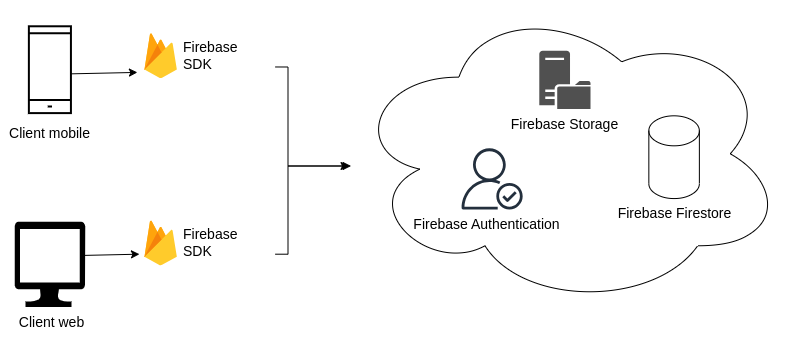
\includegraphics[width=\textwidth]{architecture}
	\caption{Présentation de l'architecture physique}
\end{figure}

\section{Technologies utilisées}
\subsection{Kotlin}
Kotlin est un langage de programmation orienté objet, à typage statique, interopérable avec la machine virtuelle Java, les bibliothèques de classes Java et Android.
Il peut être utilisé presque partout où Java est utilisé, pour le développement côté serveur, les applications Android et bien plus encore. Kotlin fonctionne parfaitement avec toutes les et s'exécute avec le même niveau de performance que Java \cite{dmitry_jemerov_kotlin}.

\subsection{Mediapipe}
MediaPipe est un outil développé par Google qui offre des outils et des modèles pour le traitement des médias en temps réel, y compris la vision par ordinateur et le suivi de mouvement. Il simplifie le déploiement des modèles de machine learning sur des périphériques tels que des smartphones avec des bibliothèques low code.
Mediapipe nous a permis d'analyser et classifier les entrées audio en temps réel en utilisant YAMNet.

\subsection{YAMNet}
YAMNet\cite{yamnet} est un réseau neuronal préformé qui utilise l'architecture de convolution séparable en profondeur MobileNetV1 \cite{andrew_g_howard_menglong_zhu_bo_chen_dmitry_kalenichenko_weijun_wang_tobias_weyand_marco_andreetto_hartwig_adam_mobilenets}. Il peut utiliser une forme d'onde audio comme entrée et faire des prédictions indépendantes pour chacun des 521 événements audio du corpus AudioSet \cite{dataset_large_scale}.

\subsection{Firebase}
Firebase est une plateforme de développement d'applications mobiles et web appartenant à Google, qui offre un ensemble de services cloud, tels que des bases de données en temps réel, l'authentification des utilisateurs, l'hébergement web, le stockage de fichiers, et des outils d'analyse avancés. Elle nous a permis de nous concentrer sur la création de fonctionnalités uniques tout en bénéficiant de la puissance du cloud pour la gestion des données et des utilisateurs ainsi que l'hébergement.

\subsection{Angular}
Angular est un framework de développement d'applications web open-source développé par Google. Il est largement utilisé pour la création d'applications web modernes et dynamiques. Angular est basé sur le langage TypeScript, une version améliorée de JavaScript, et offre un ensemble complet de fonctionnalités pour simplifier le développement front-end.

\section{Diagramme de déploiement}
\begin{figure}[H]
	\centering
	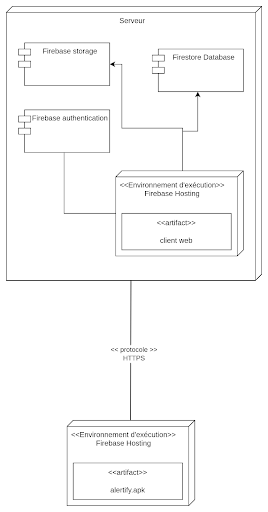
\includegraphics[height=500px]{deploiement}
	\caption{Diagramme de déploiement}
\end{figure}

\section{Expérience utilisateur et fonctionnement}
\subsection{Expérience utilisateur}
Le processus de conception de l'expérience utilisateur consiste à s'assurer qu'aucun aspect de l'expérience de l'utilisateur avec une solution ne se produit sans l’intention consciente et explicite de ce dernier. Cela signifie qu'il faut prendre en compte chaque possibilité de chaque action que l'utilisateur est susceptible de faire et de comprendre ses attentes à chaque étape du processus \cite{jesse_james_garrett_elements}.\\

Dans le cadre de notre travail, l'attention portée à l'UX est cruciale pour garantir l'adoption et l'efficacité du système par les utilisateurs finaux.

Tout d'abord, il est essentiel de comprendre les besoins, les compétences techniques et les préférences des utilisateurs potentiels à Lubumbashi. Cette compréhension approfondie permettra de concevoir une interface utilisateur conviviale et intuitive, adaptée au contexte local. Il est crucial que l'application soit facile à comprendre et à utiliser, même pour les utilisateurs peu familiers avec les technologies modernes.

\subsection{Fonctionnement}

Pour permettre à notre application mobile de fonctionner, nous avons recouru au composant d’application appelé service. Un service est un composant d'application qui peut effectuer des opérations de longue durée en arrière-plan. Il ne fournit pas d'interface utilisateur. Une fois lancé, un service peut continuer à fonctionner pendant un certain temps, même après que l'utilisateur a basculé vers une autre application \cite{services}. Mais avant tout, nous devrions commencer par demander la permission d'accéder à la géolocalisation ainsi qu'au périphérique audio du smartphone, notamment le microphone.

Une fois que l'application a obtenu l'accès au microphone, les données captées sont évaluées à l'aide de MediaPipe. MediaPipe à pour objectif de détecter des bruits tels que les pleurs et les gémissements, qui peuvent indiquer qu'une personne est en danger. Ces scénarios déclenchent alors le lancement d'alertes. Les alertes entraînent l'envoi de messages contenant la géolocalisation du smartphone aux contacts préenregistrés, ainsi qu'au serveur backend, dans le cas où le smartphone dispose d'une connexion Internet. Également, l'utilisateur peut envoyer l'alerte manuellement d'une manière discrète en appuyant trois fois ou plus sur l'une des touches physiques de volume de son smartphone, cette action est détectée par le ContentObserver\cite{content_observer}.

\begin{figure}[H]
	\centering
	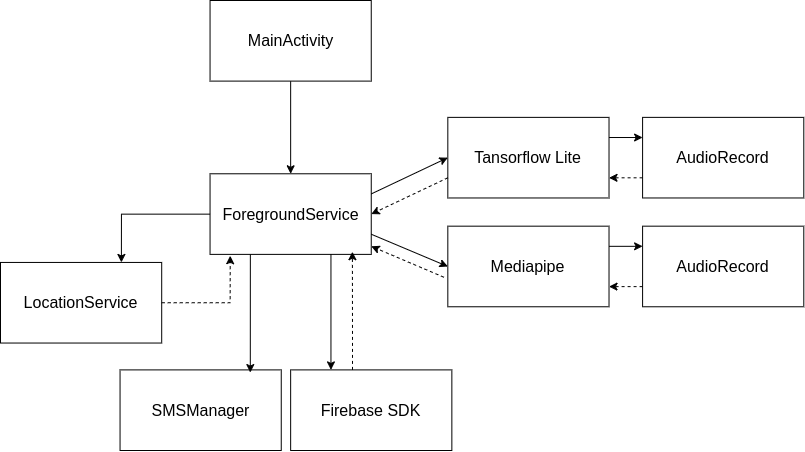
\includegraphics[width=\textwidth]{fonctionnement}
	\caption{Communication des différentes composantes lors de l’envoi d’une alerte}
\end{figure}

\begin{figure}[H]
	\centering
	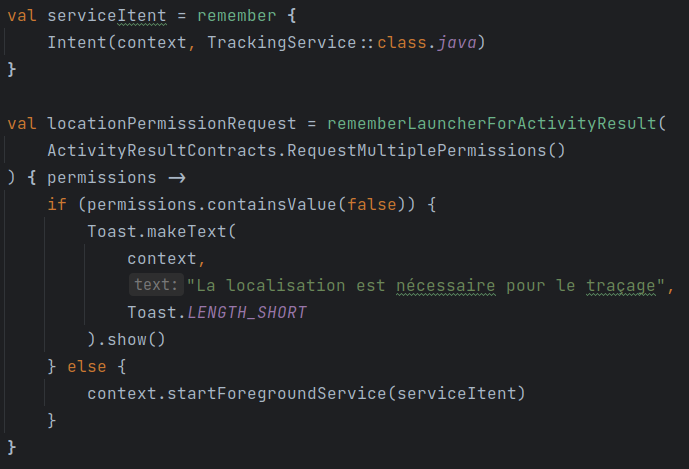
\includegraphics[width=\textwidth]{code_permission}
	\caption{Demande de permission et lancement du service TrackingService}
\end{figure}

\begin{figure}[H]
	\centering
	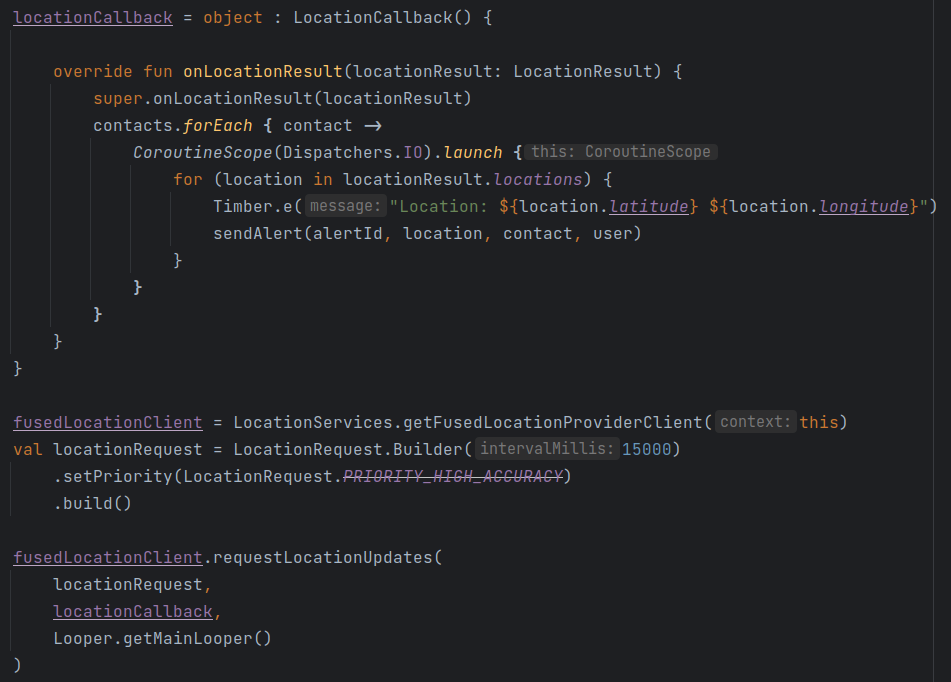
\includegraphics[width=\textwidth]{code_location}
	\caption{Récupération de la localisation}
\end{figure}

\begin{figure}[H]
	\centering
	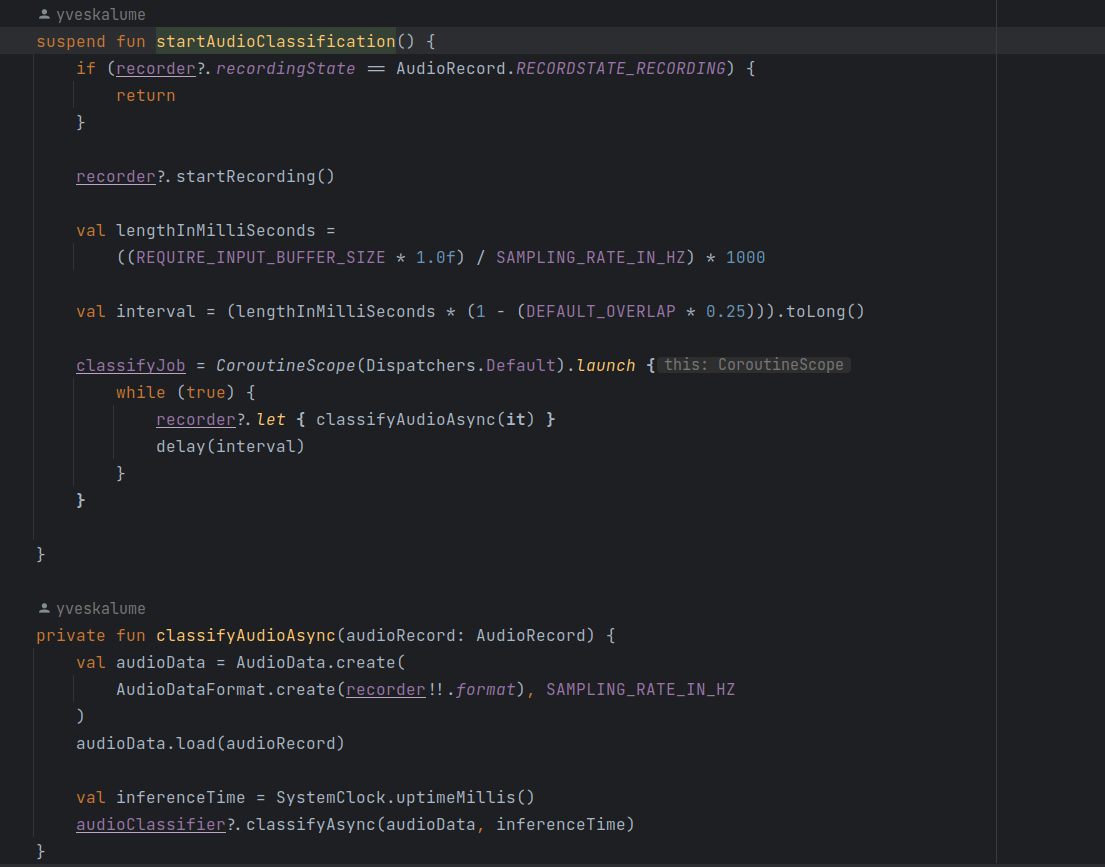
\includegraphics[width=\textwidth]{code_classification}
	\caption{Classification des entrées sonores}
\end{figure}

\begin{figure}[H]
	\centering
	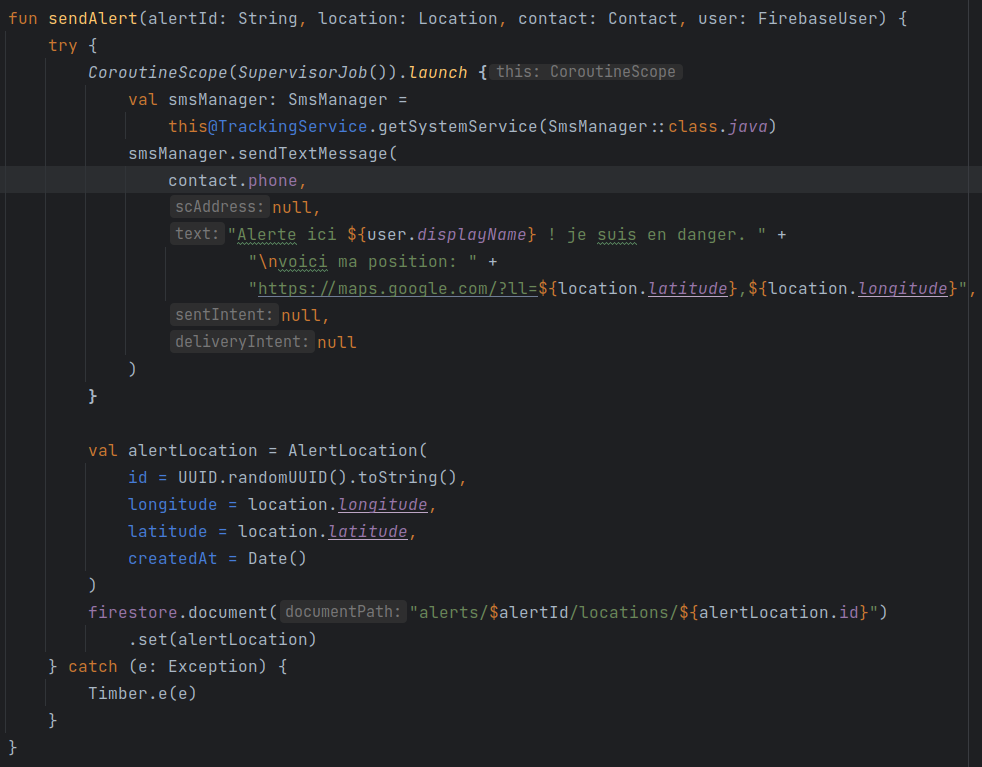
\includegraphics[width=\textwidth]{code_envoi_alerte}
	\caption{Envois d’alertes}
\end{figure}

\section{Captures d’écrans}
\subsection{Client mobile pour utilisateur}

\begin{figure}[H]
	\centering
	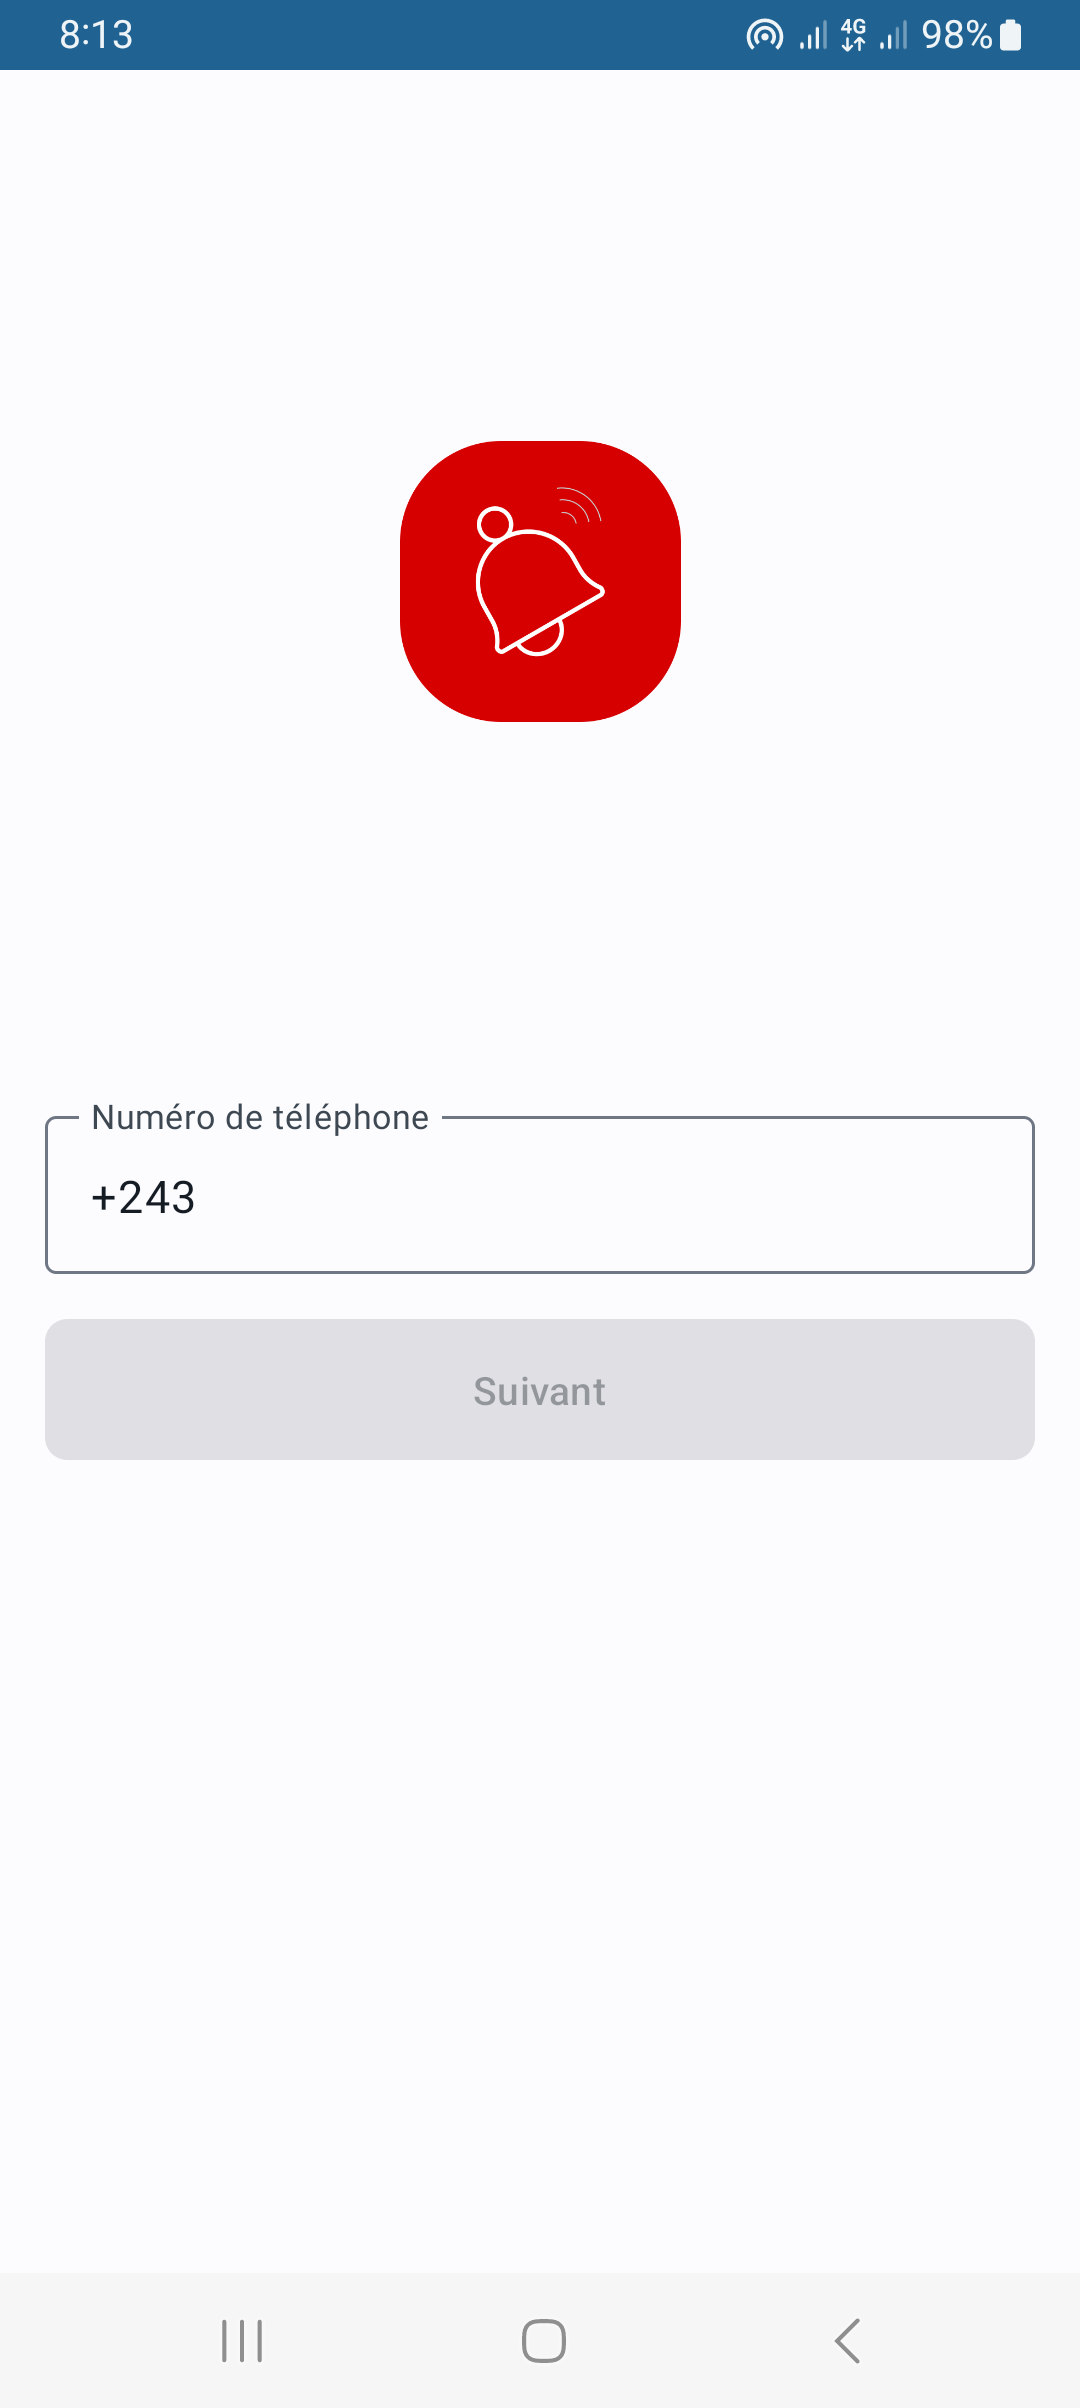
\includegraphics[width=3.6in,frame]{phone}
	\caption{Écran d’enregistrement du numéro de l’utilisateur}
\end{figure}

\begin{figure}[H]
	\centering
	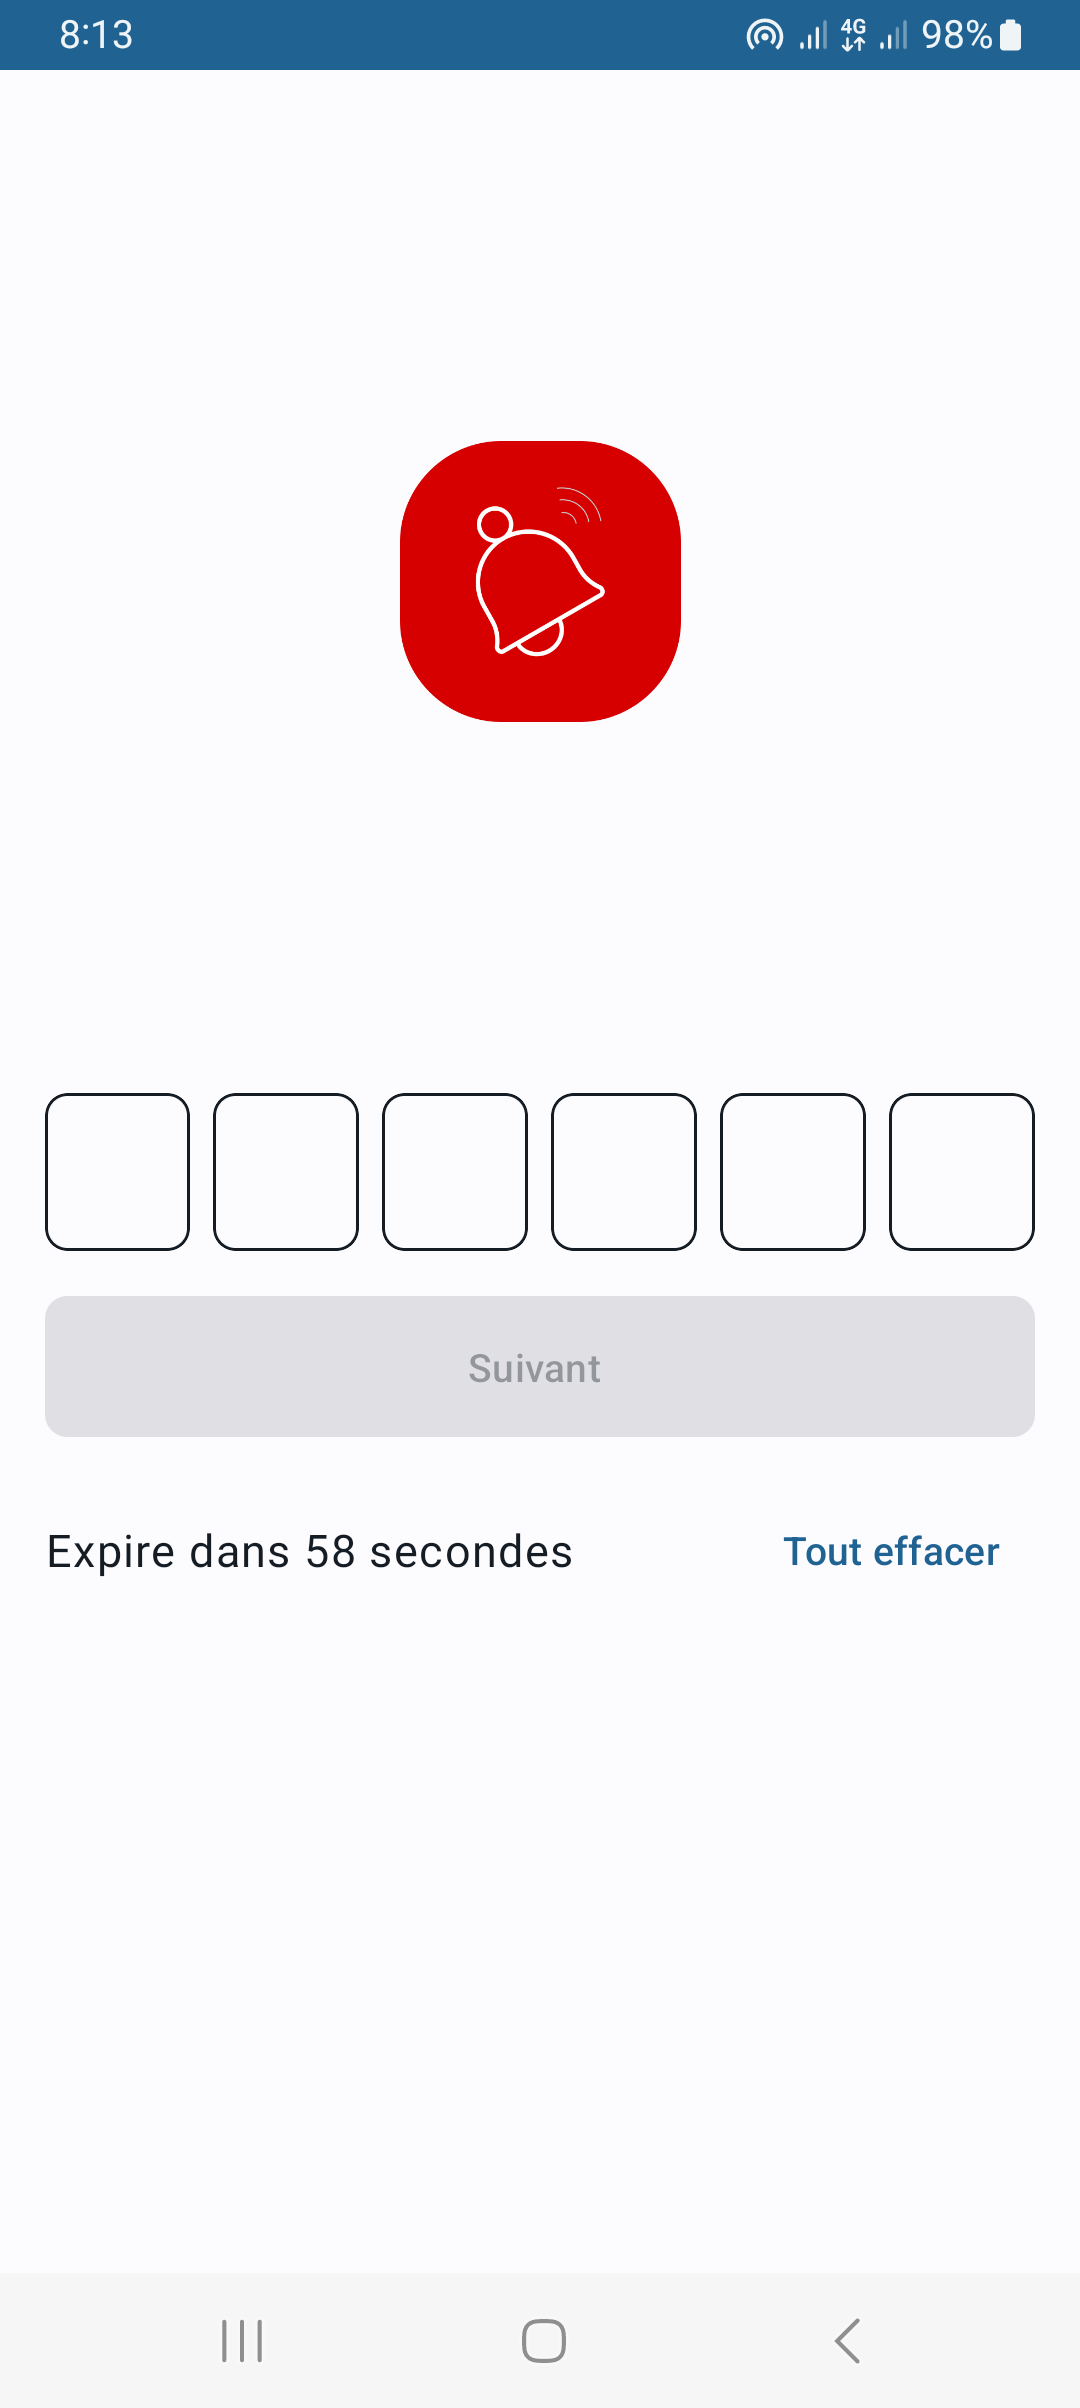
\includegraphics[width=3.6in,frame]{otp}
	\caption{Écran de soumission du code de confirmation}
\end{figure}

\begin{figure}[H]
	\centering
	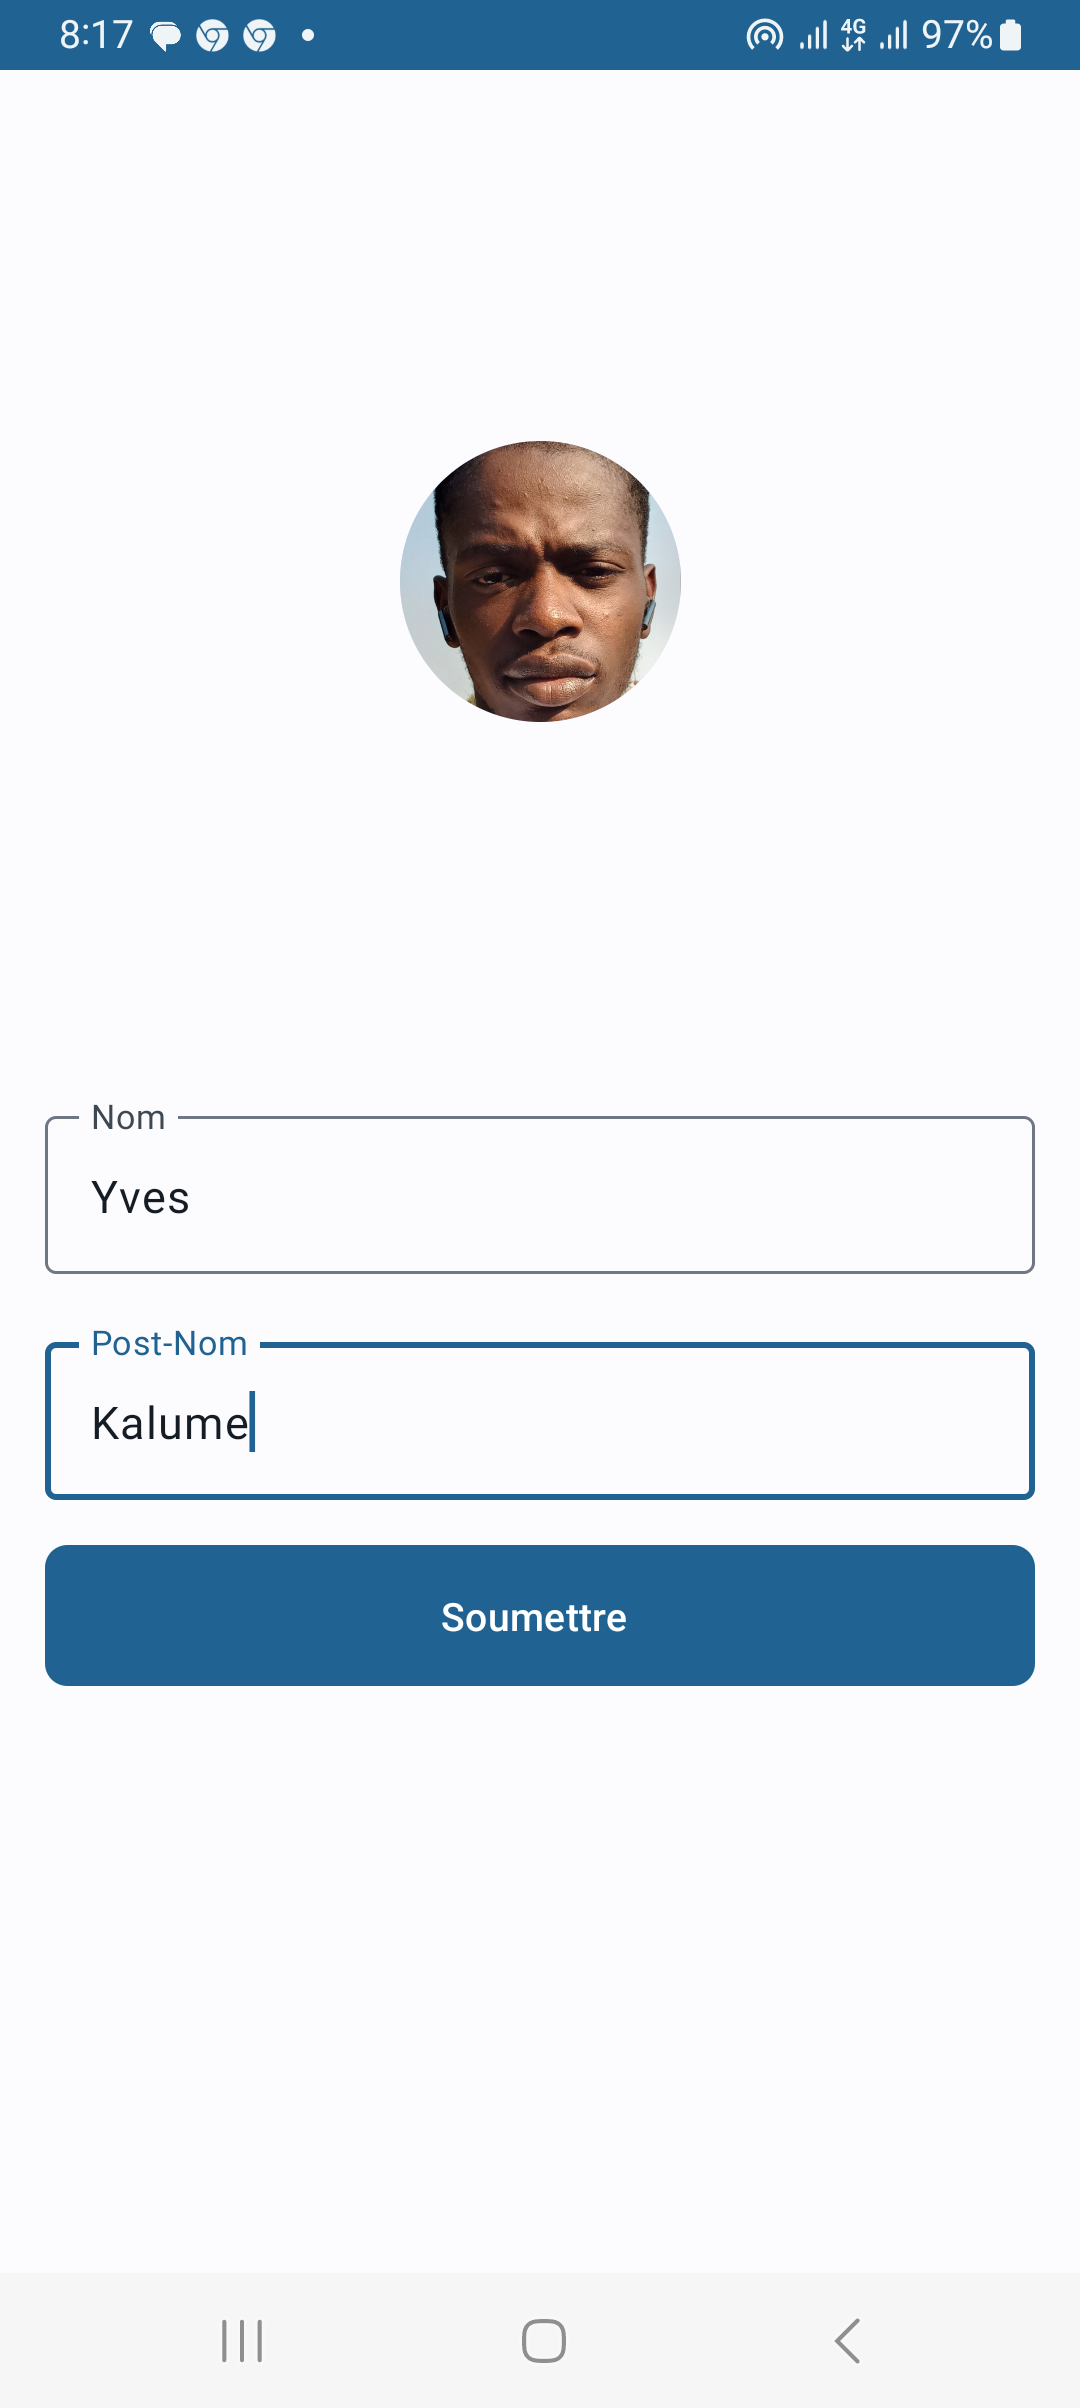
\includegraphics[width=3.6in,frame]{profile}
	\caption{Écran d’enregistrement de l’identité de l’utilisateur}
\end{figure}

\begin{figure}[H]
	\centering
	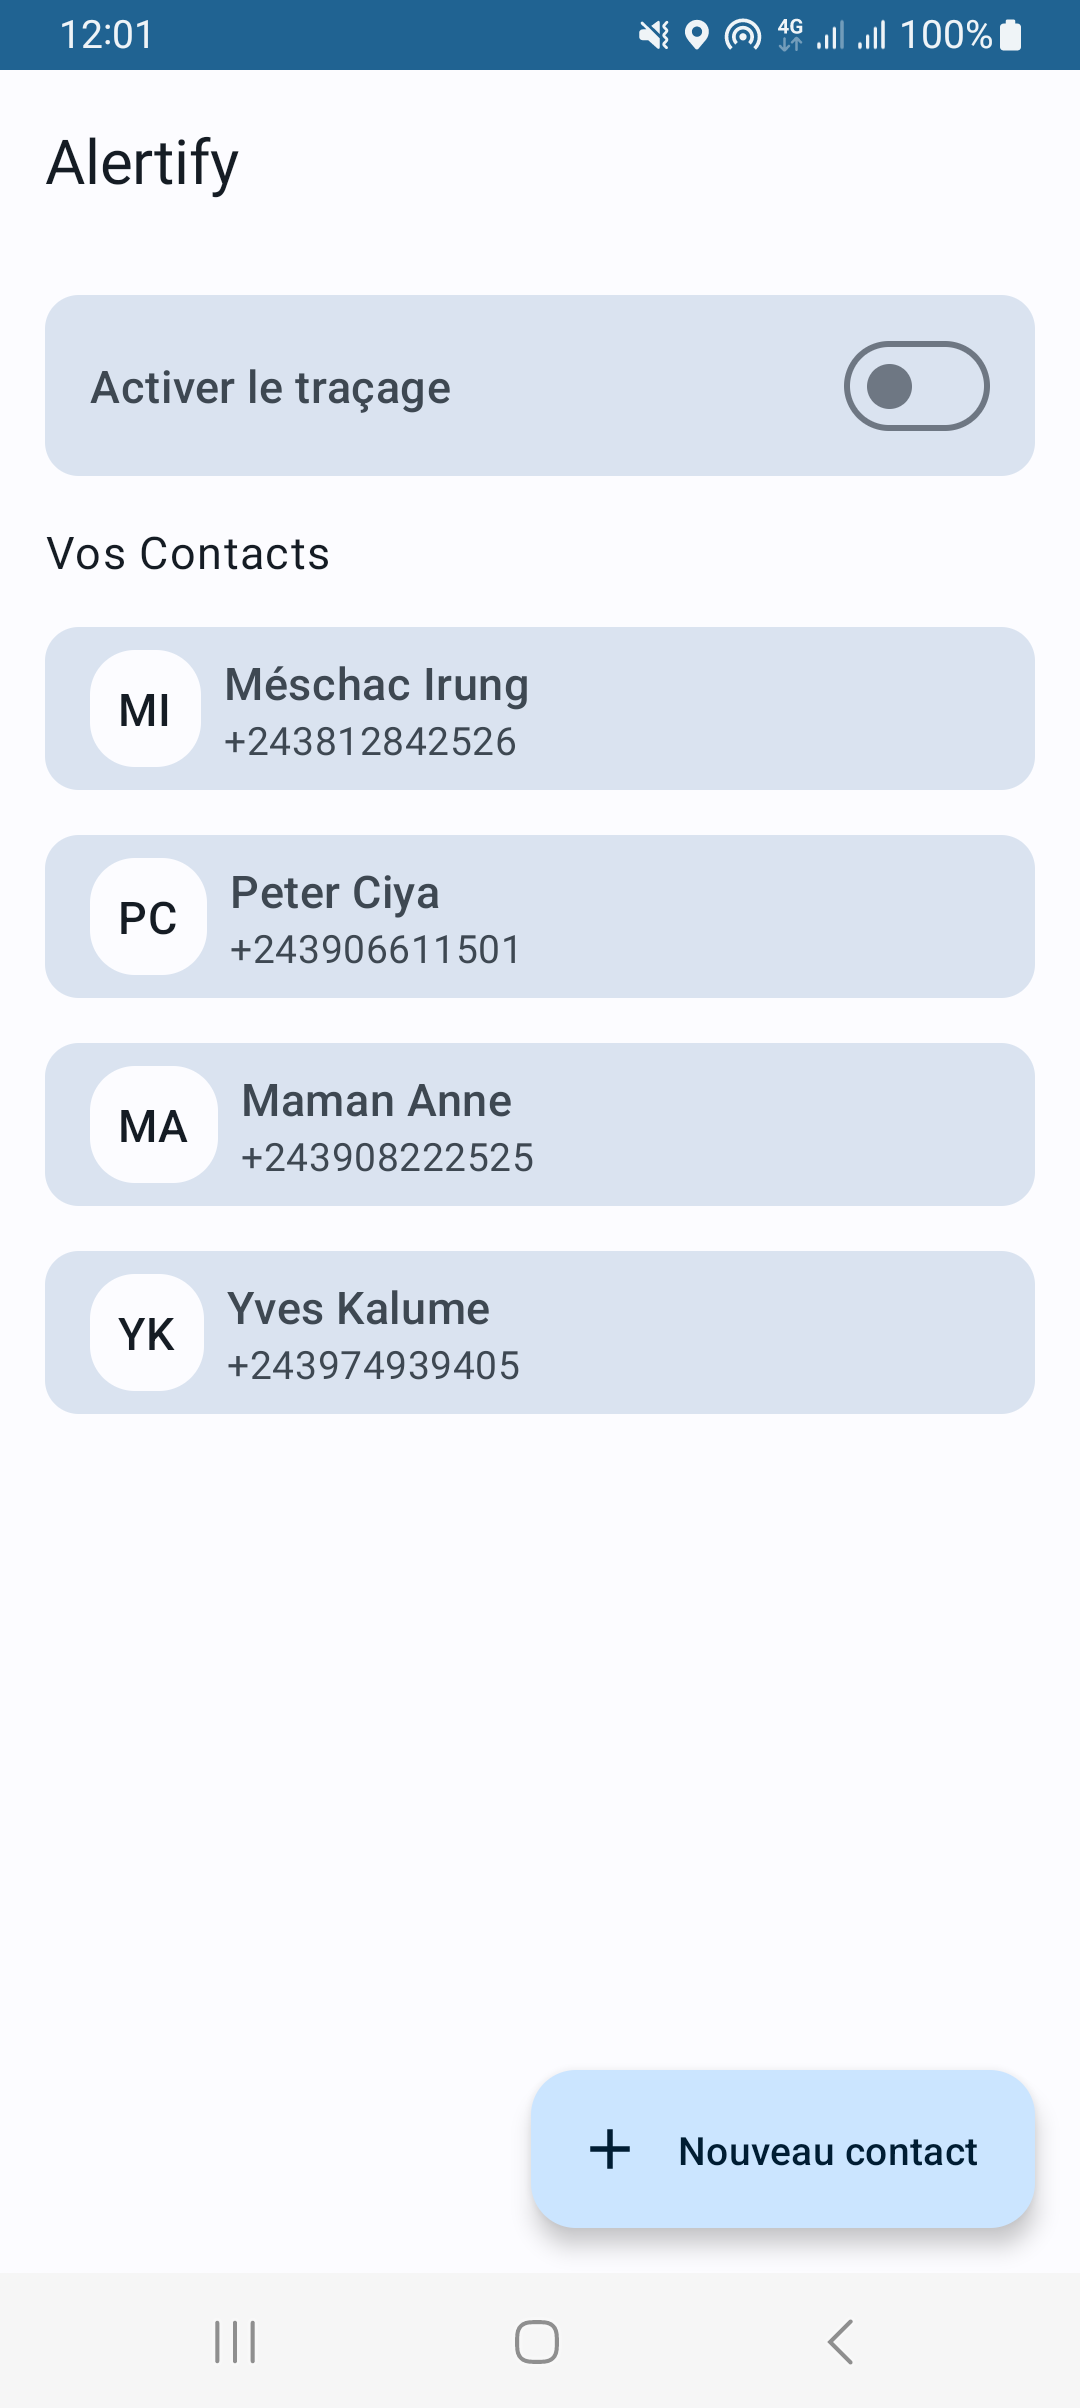
\includegraphics[width=3.6in,frame]{home}
	\caption{Écran principal}
\end{figure}

\begin{figure}[H]
	\centering
	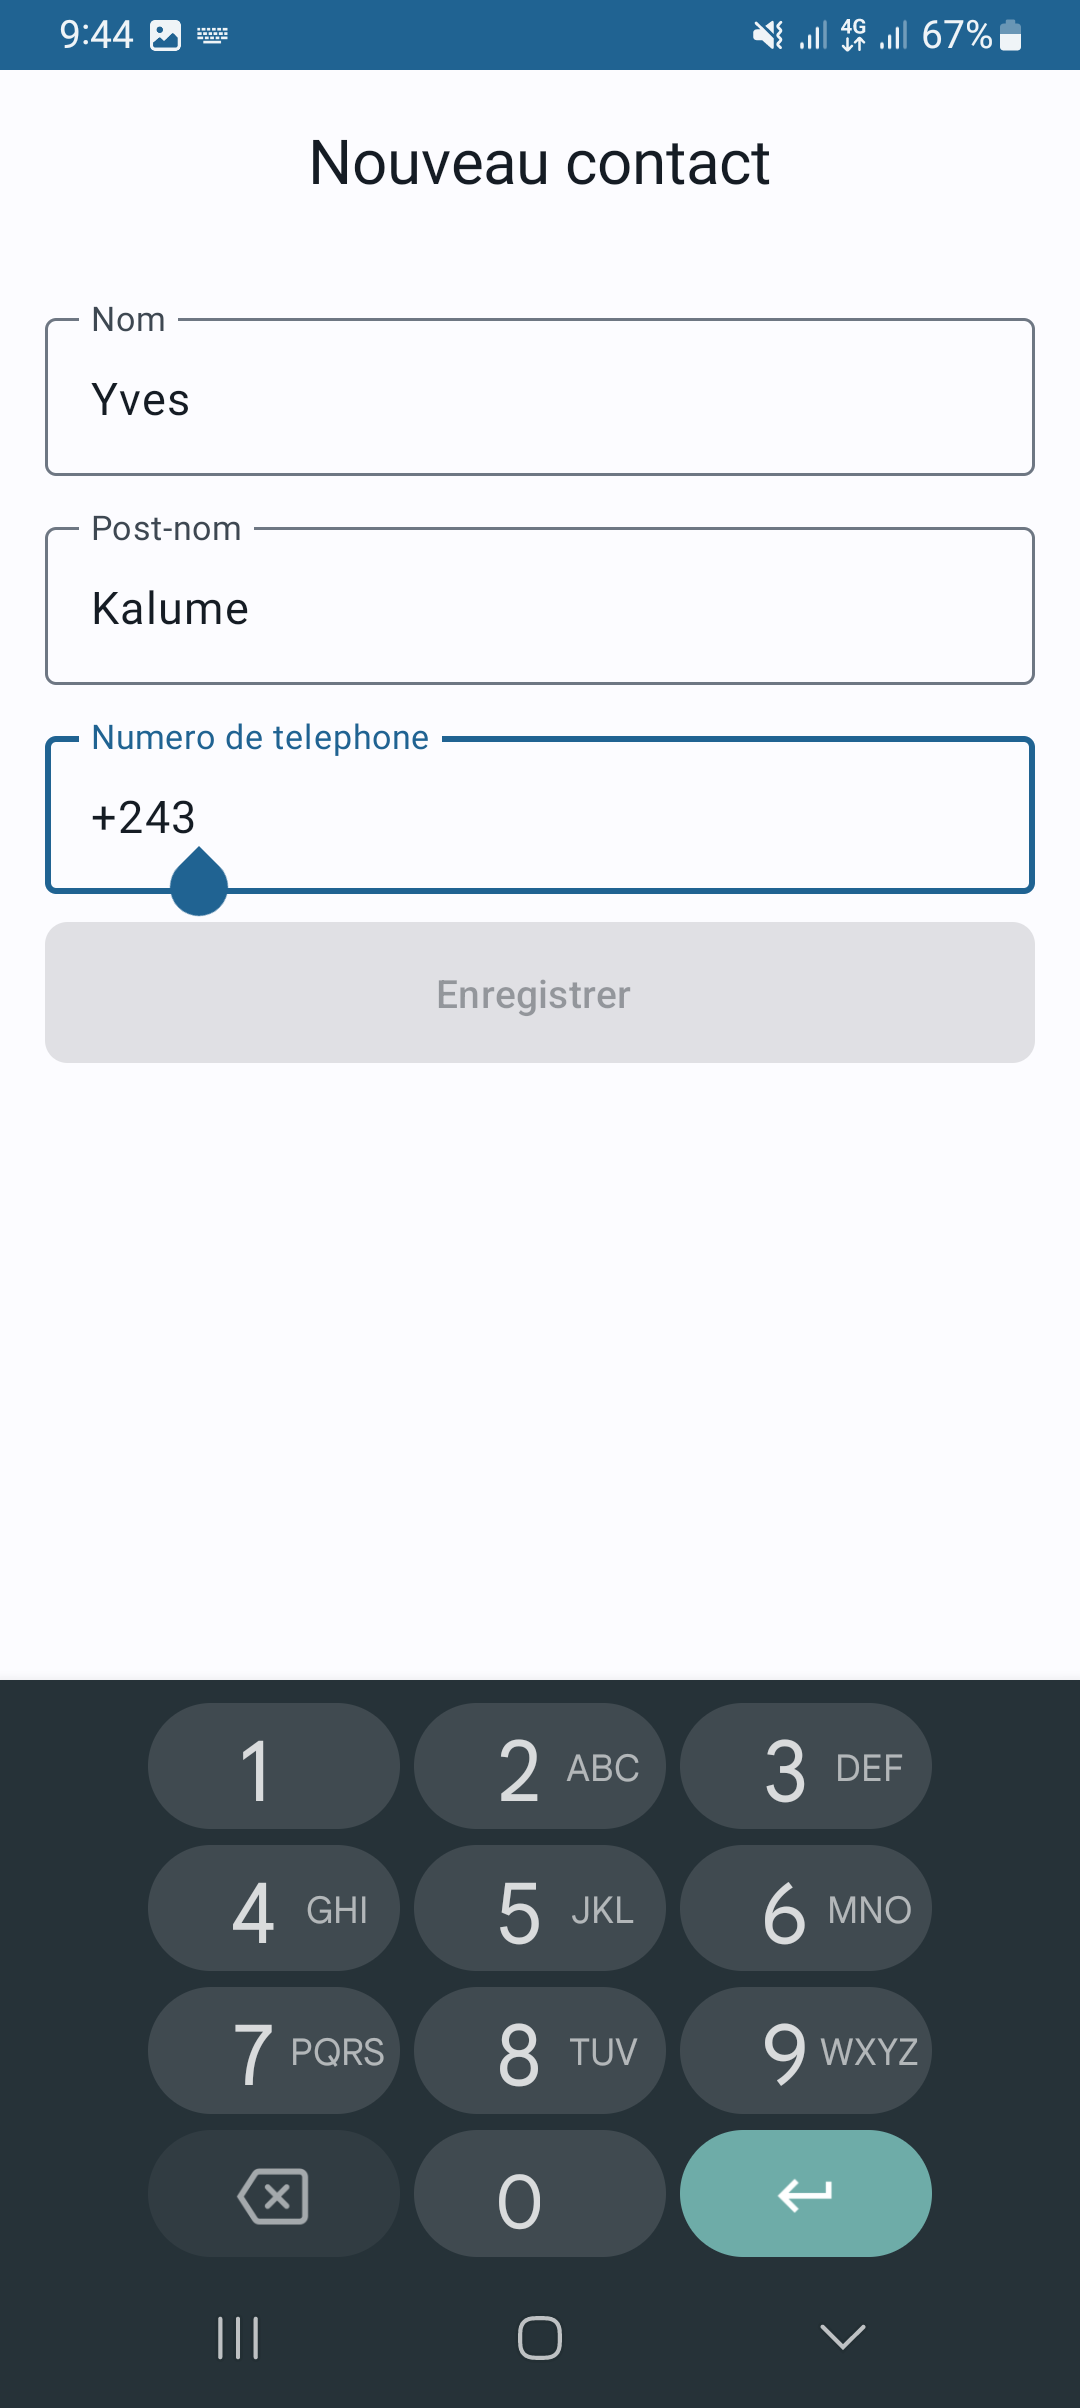
\includegraphics[width=3.6in,frame]{add_contact}
	\caption{Écran permettant d’ajouter un contact}
\end{figure}

\begin{figure}[H]
	\centering
	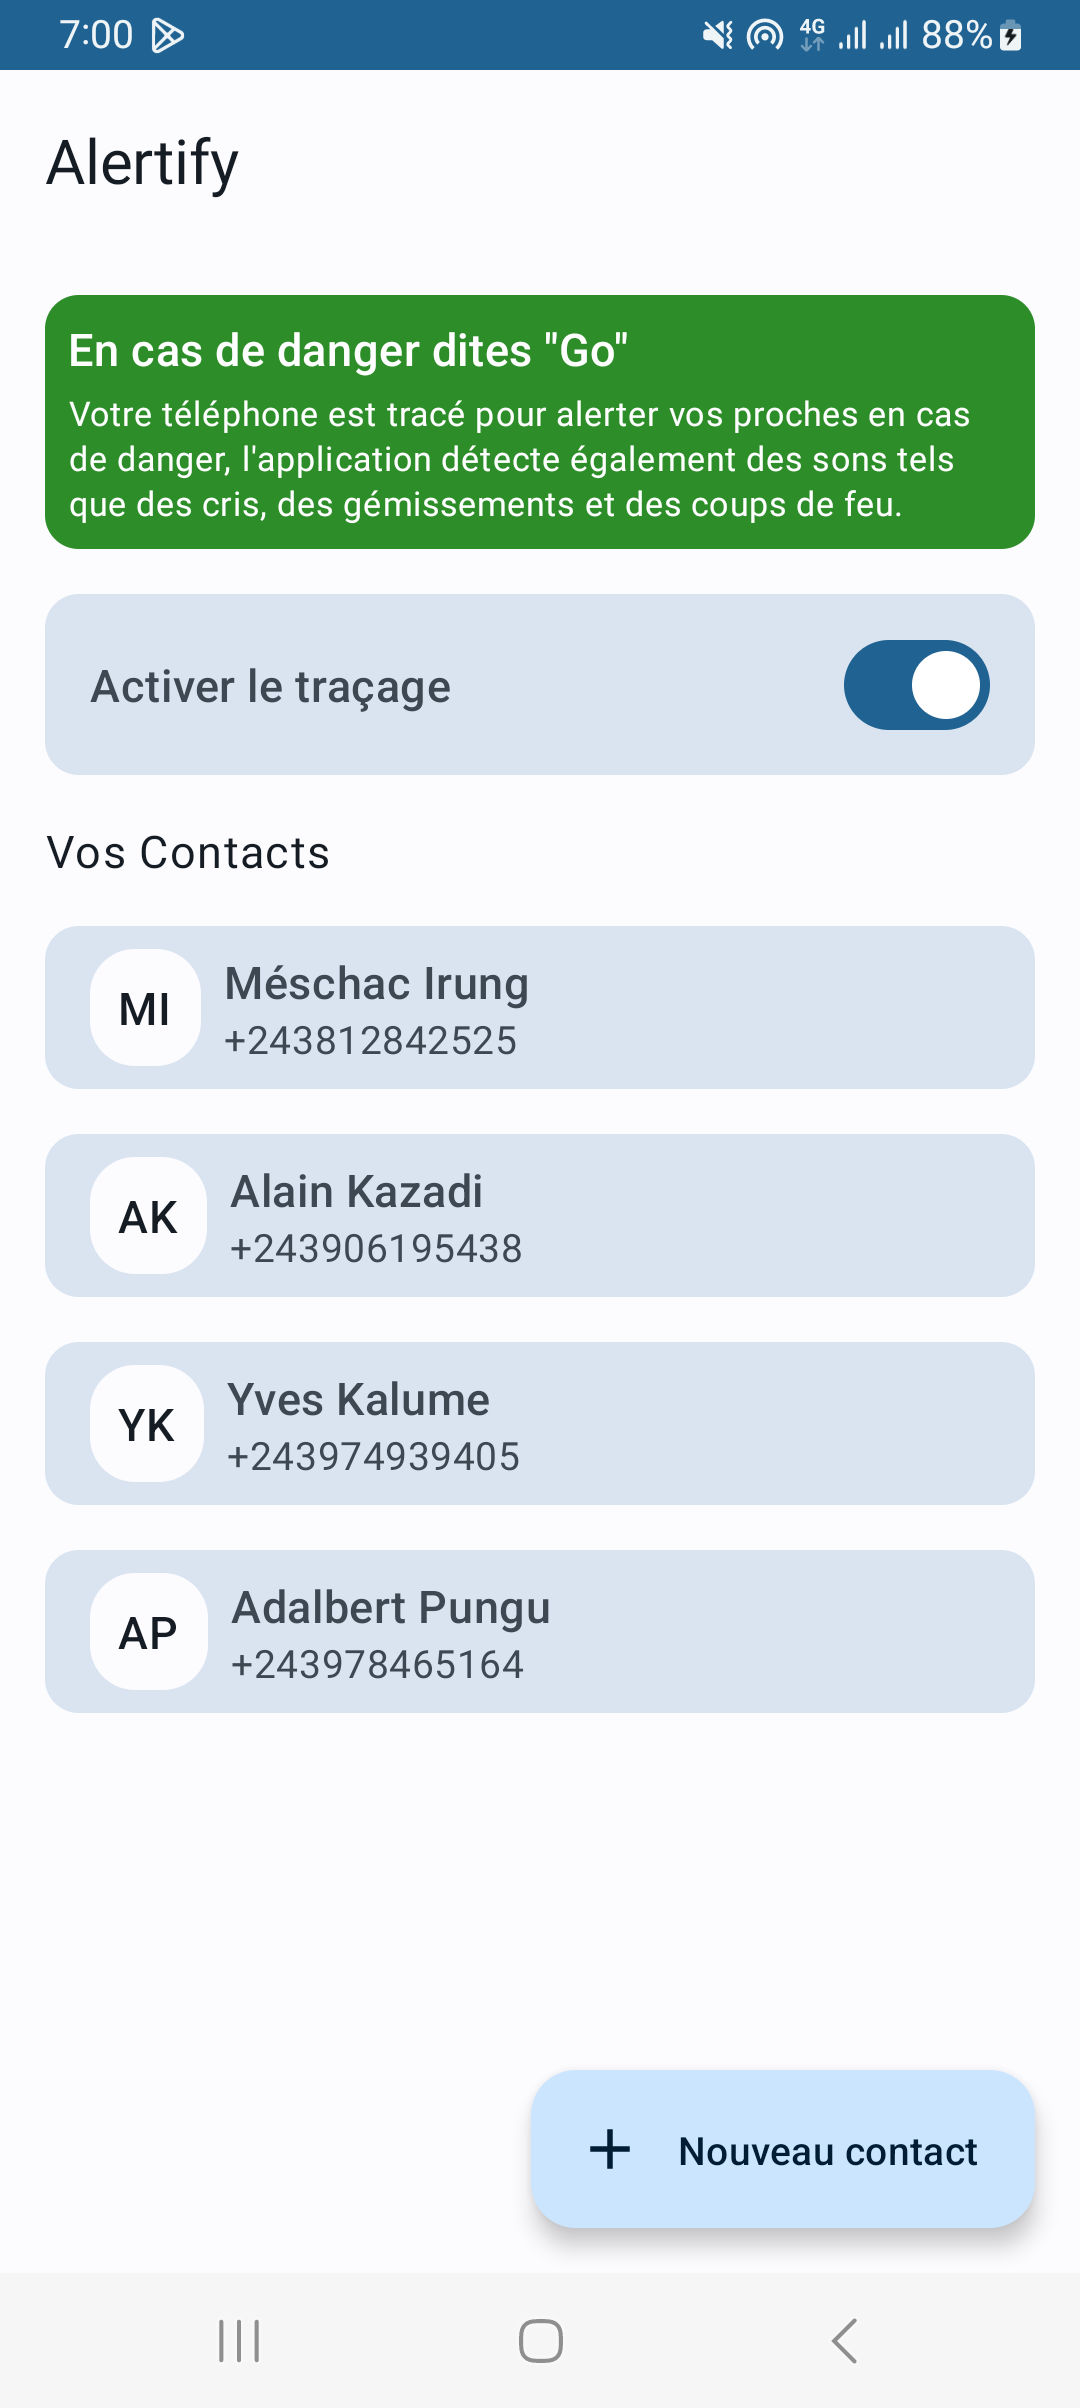
\includegraphics[width=3.6in,frame]{trackingenabled}
	\caption{Écran d'accueil, tracking activé}
\end{figure}

\begin{figure}[H]
	\centering
	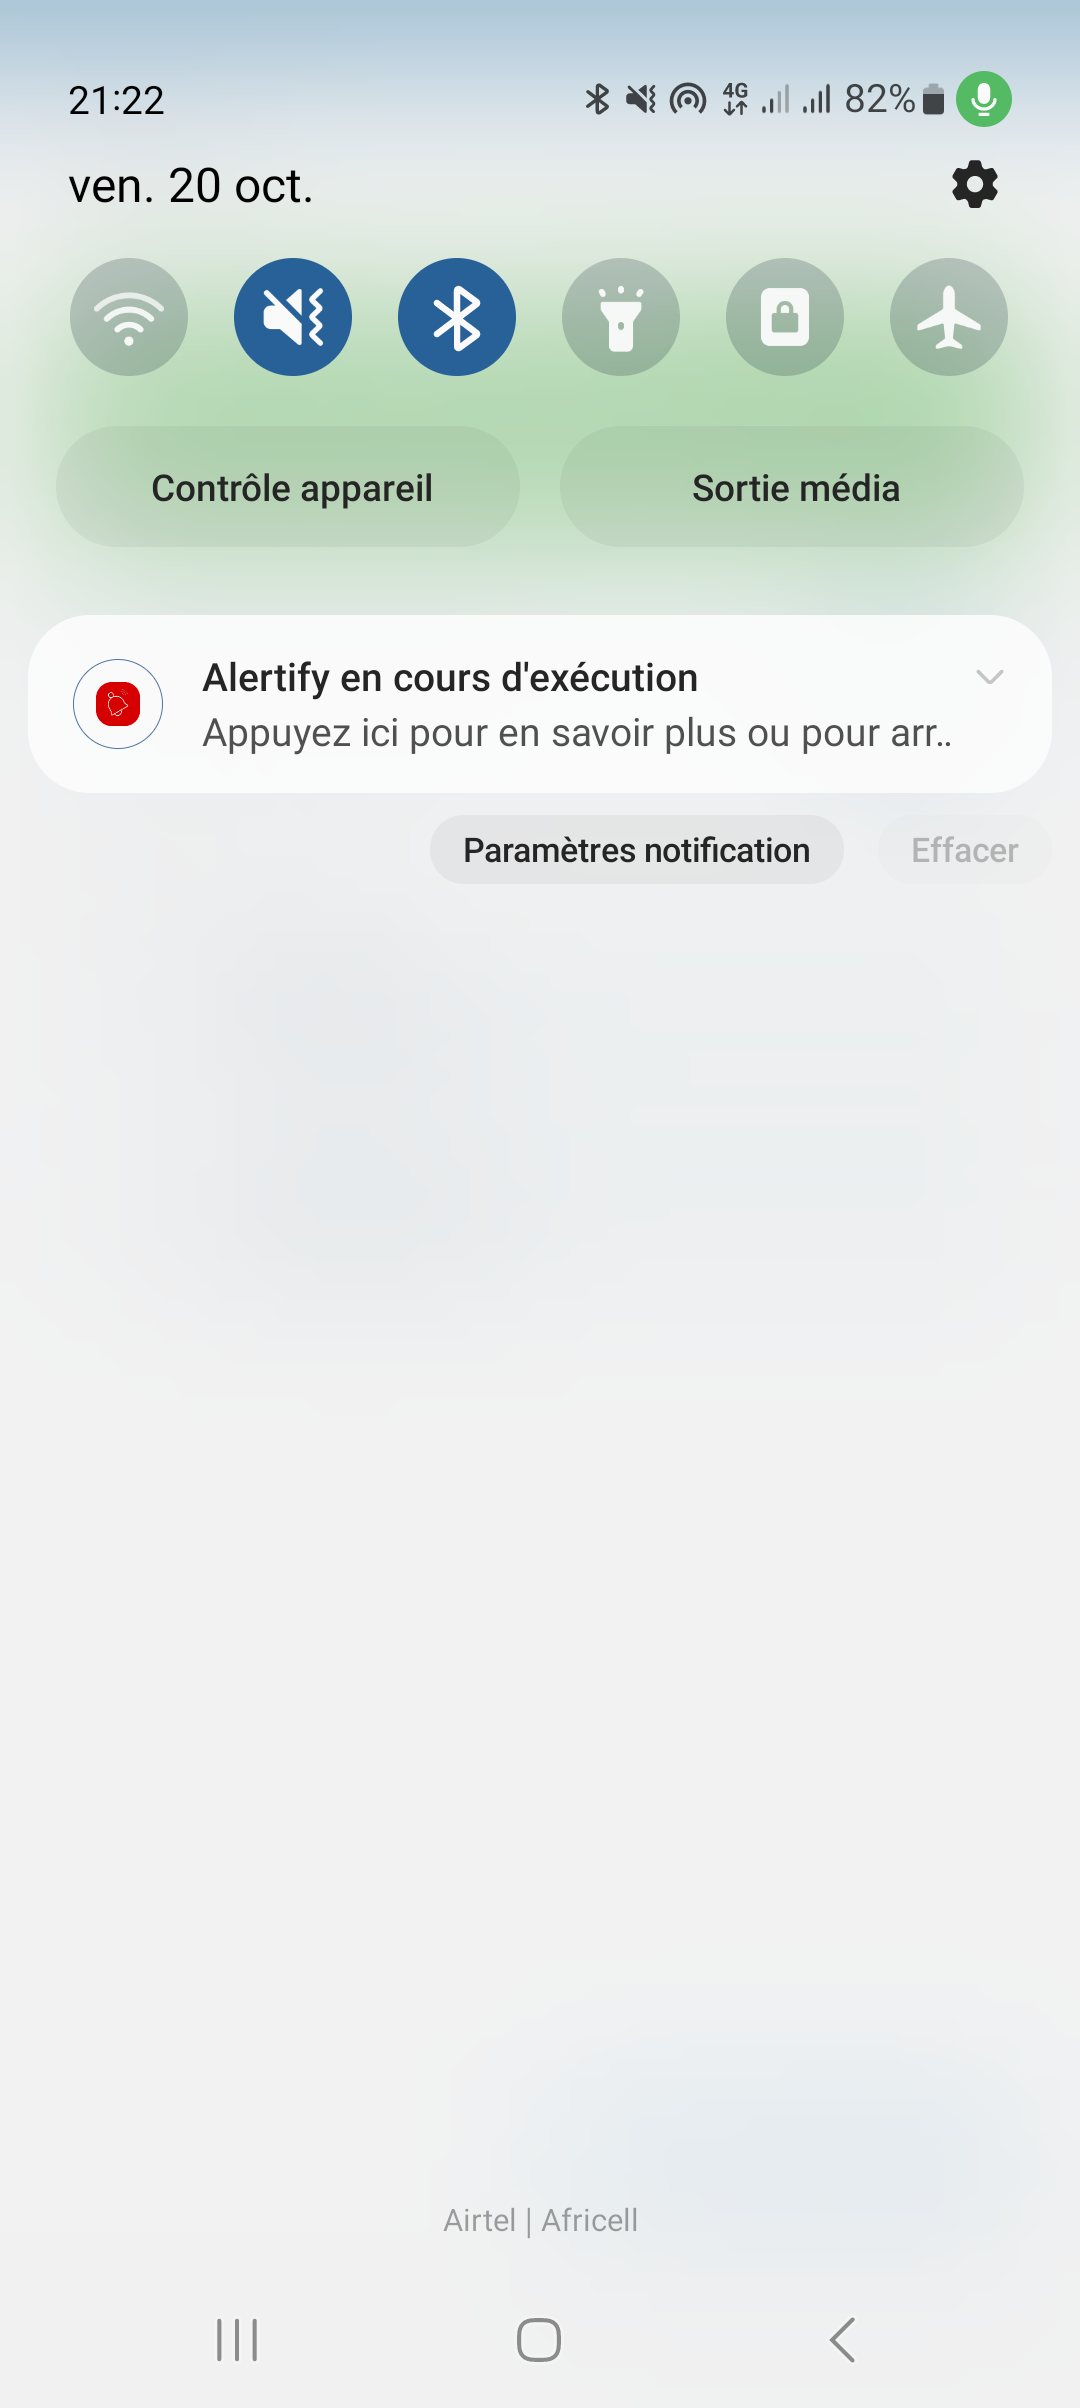
\includegraphics[width=3.6in,frame]{foreground}
	\caption{Notification signalant que le tracking est en cours}
\end{figure}

\begin{figure}[H]
	\centering
	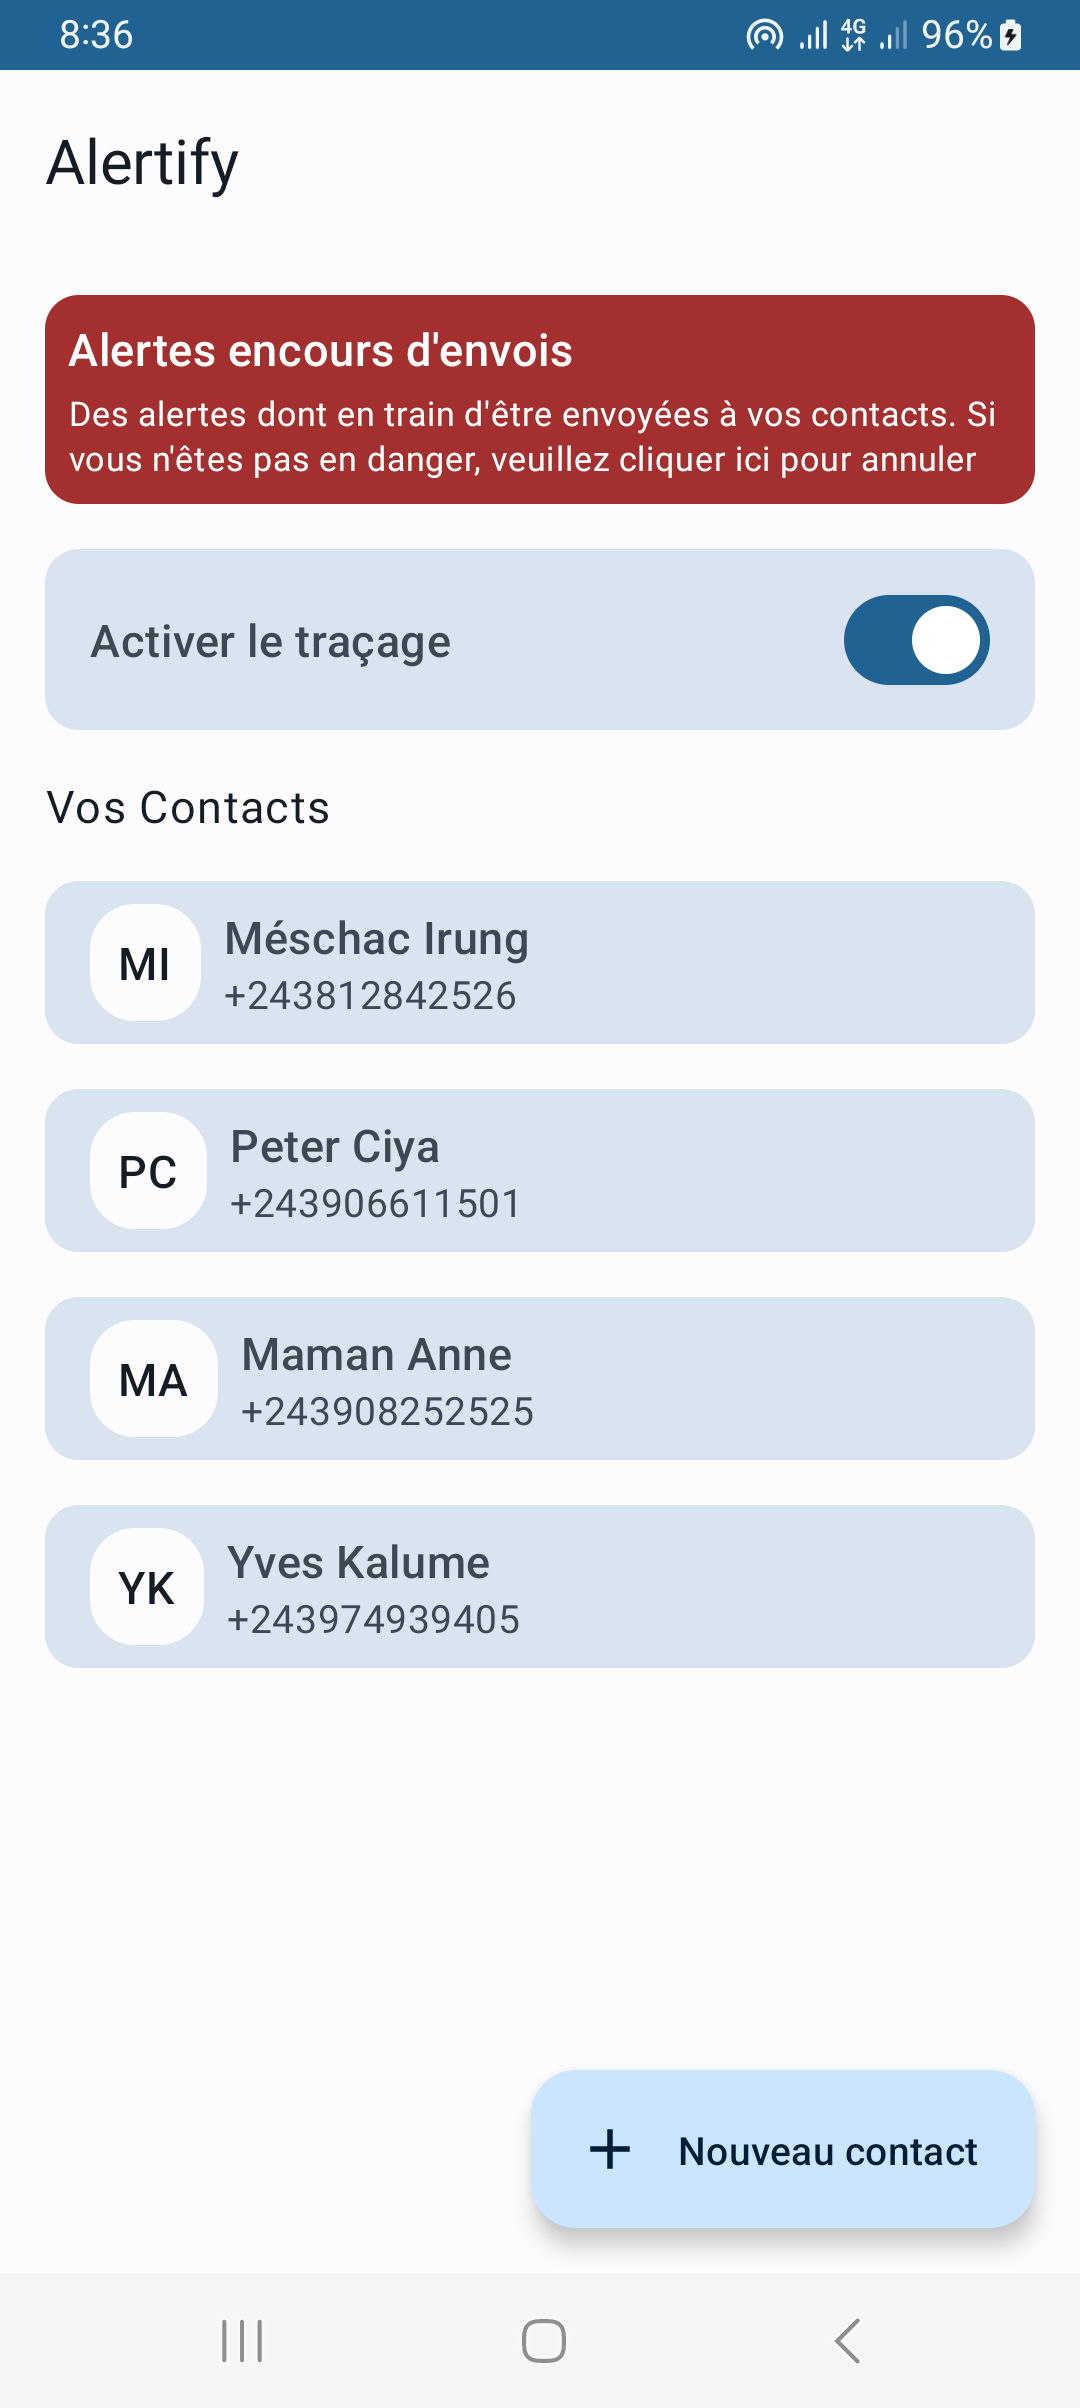
\includegraphics[width=3.6in,frame]{sendingalerts}
	\caption{Écran principal, alertes en cours d’envoi}
\end{figure}

\begin{figure}[H]
	\centering
	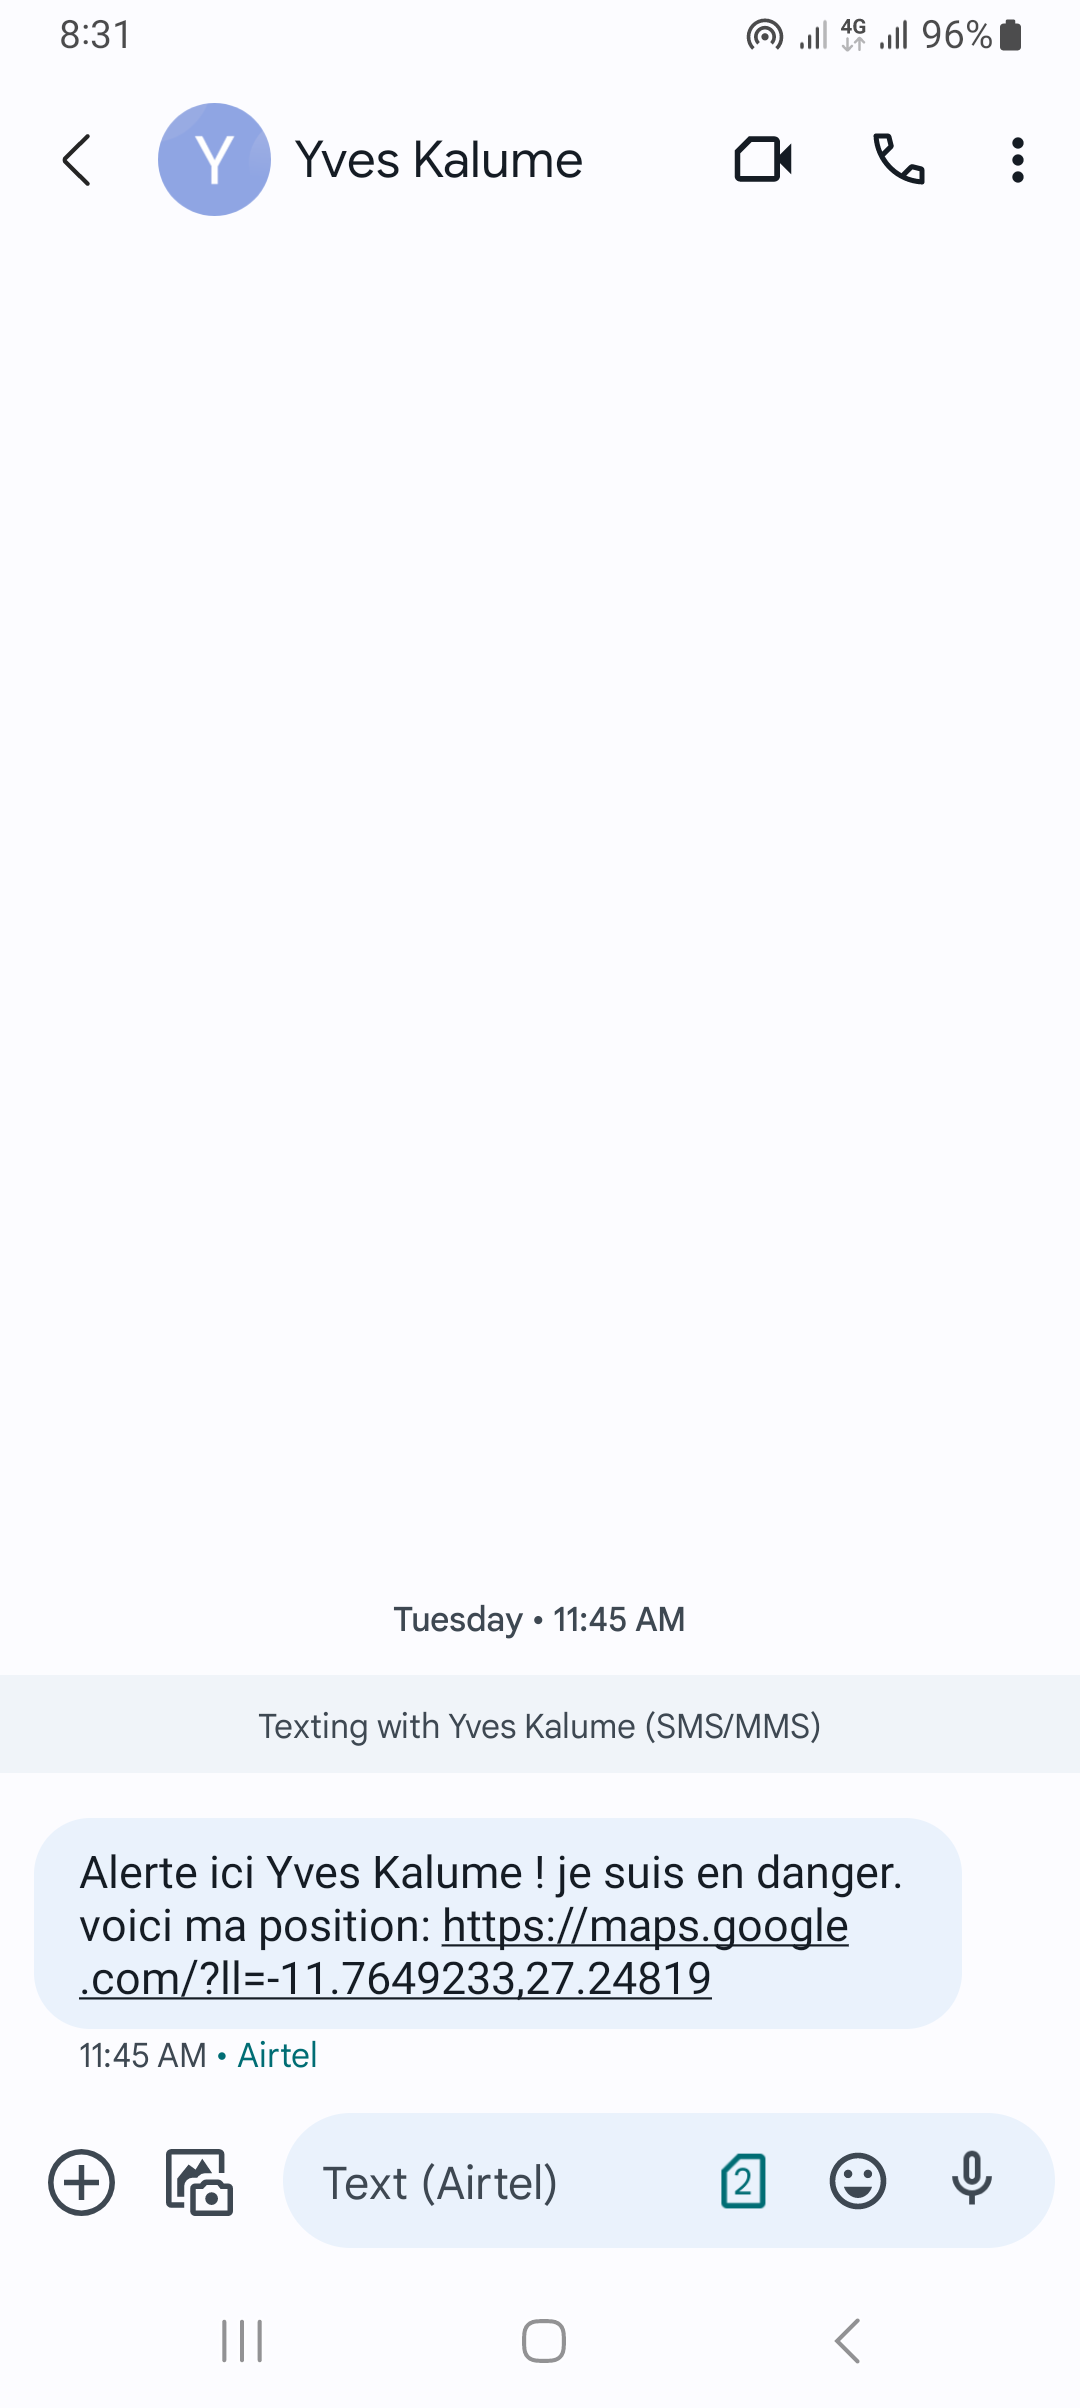
\includegraphics[width=3.6in,frame]{sms}
	\caption{SMS d’alerte}
\end{figure}

\subsection{Client web pour administrateur}

\begin{figure}[H]
	\centering
	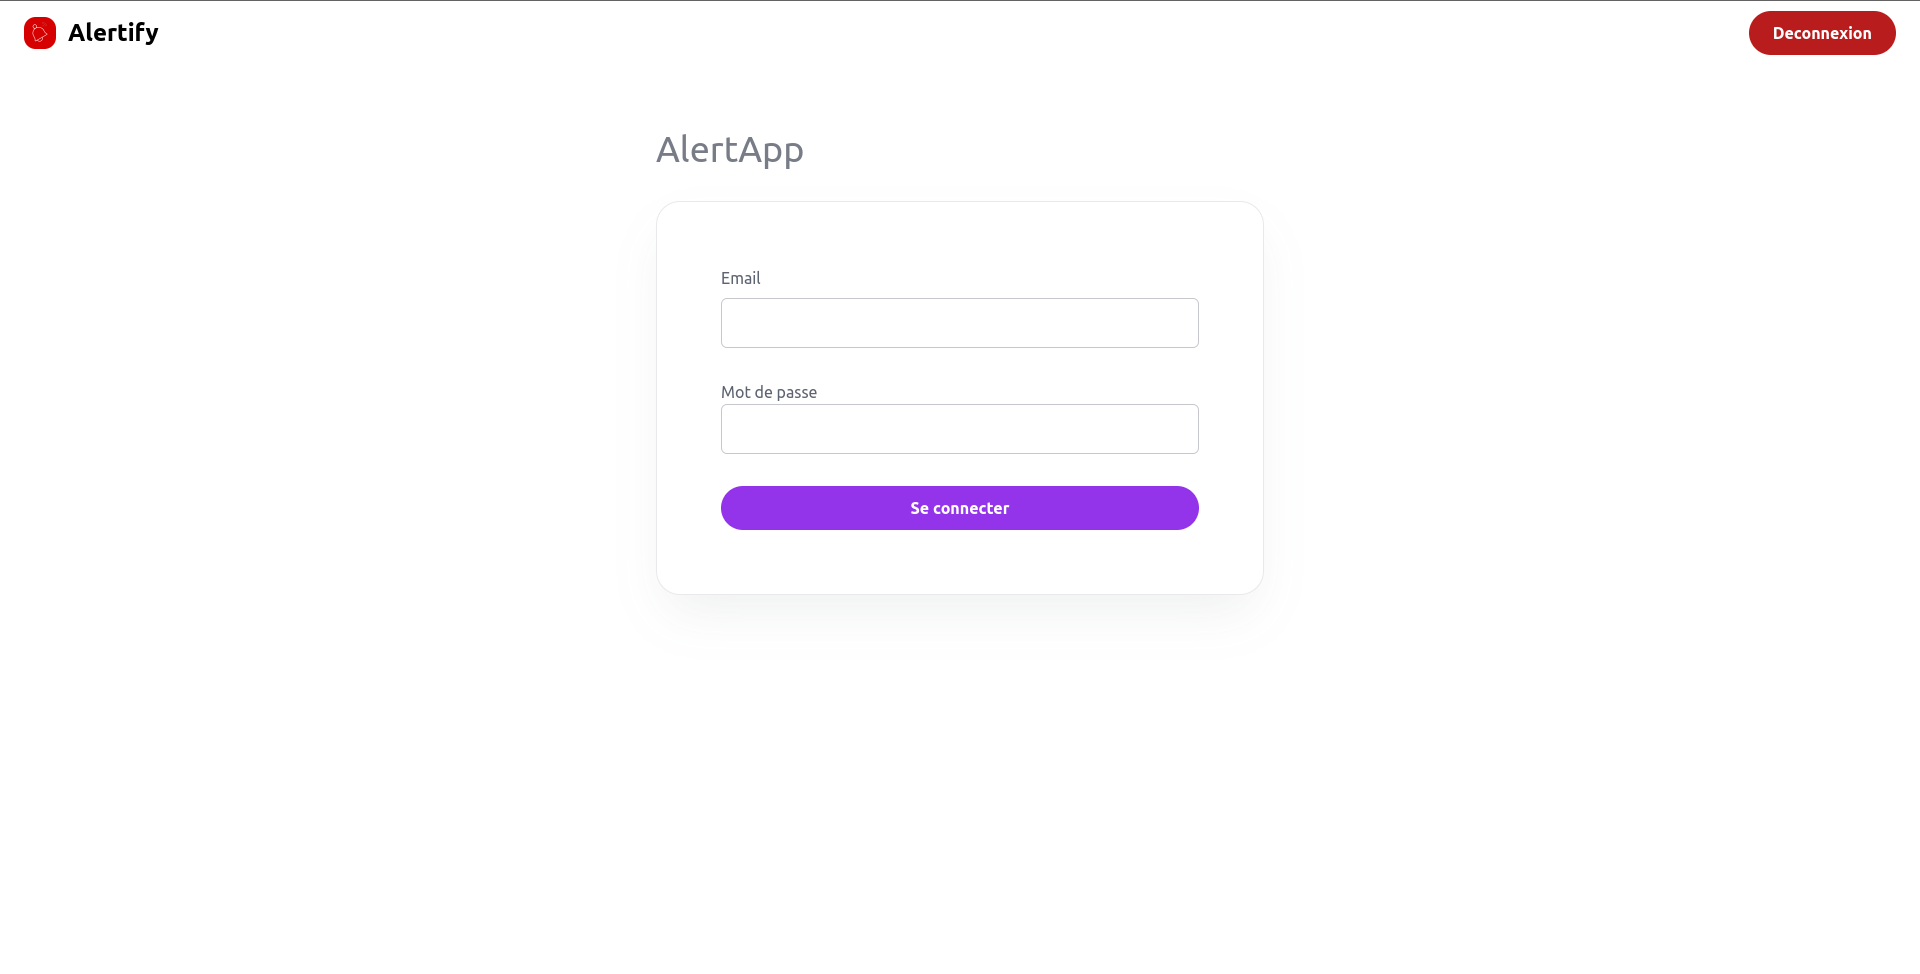
\includegraphics[width=\textwidth,frame]{admin_auth}
	\caption{Page de connexion administrateur}
\end{figure}

\begin{figure}[H]
	\centering
	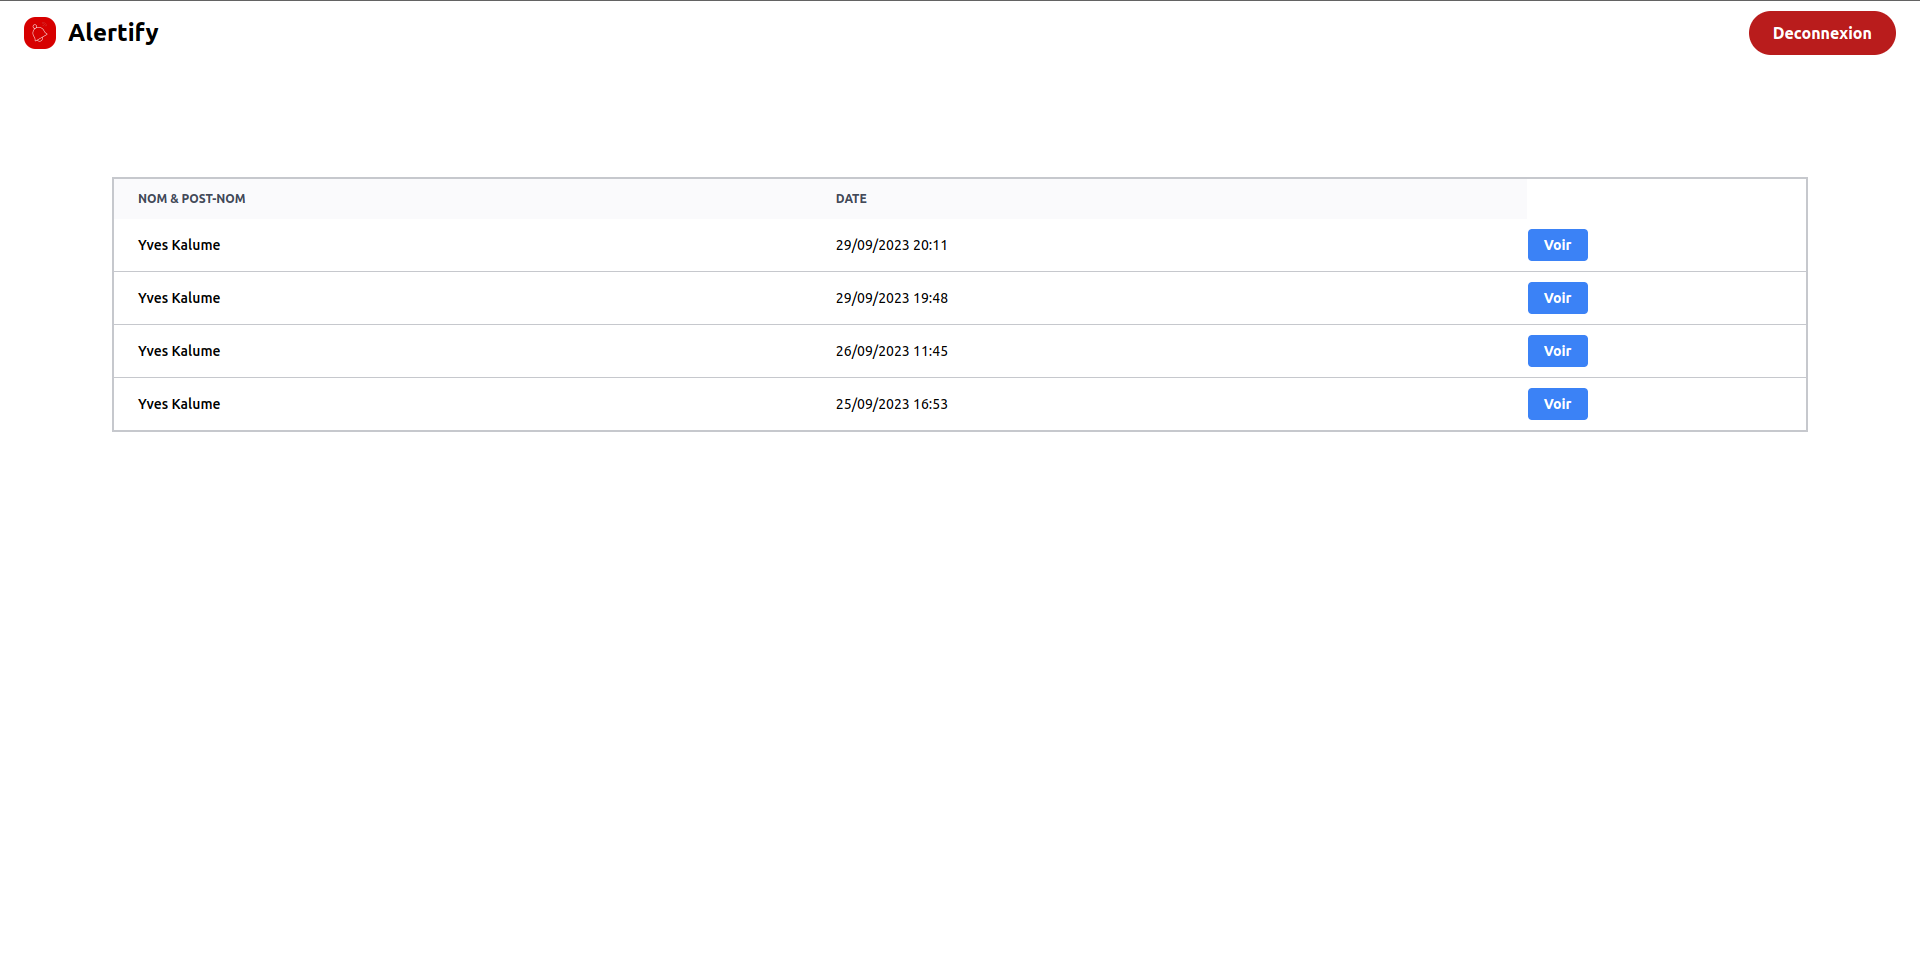
\includegraphics[width=\textwidth,frame]{admin_home}
	\caption{Listes des alertes}
\end{figure}

\begin{figure}[H]
	\centering
	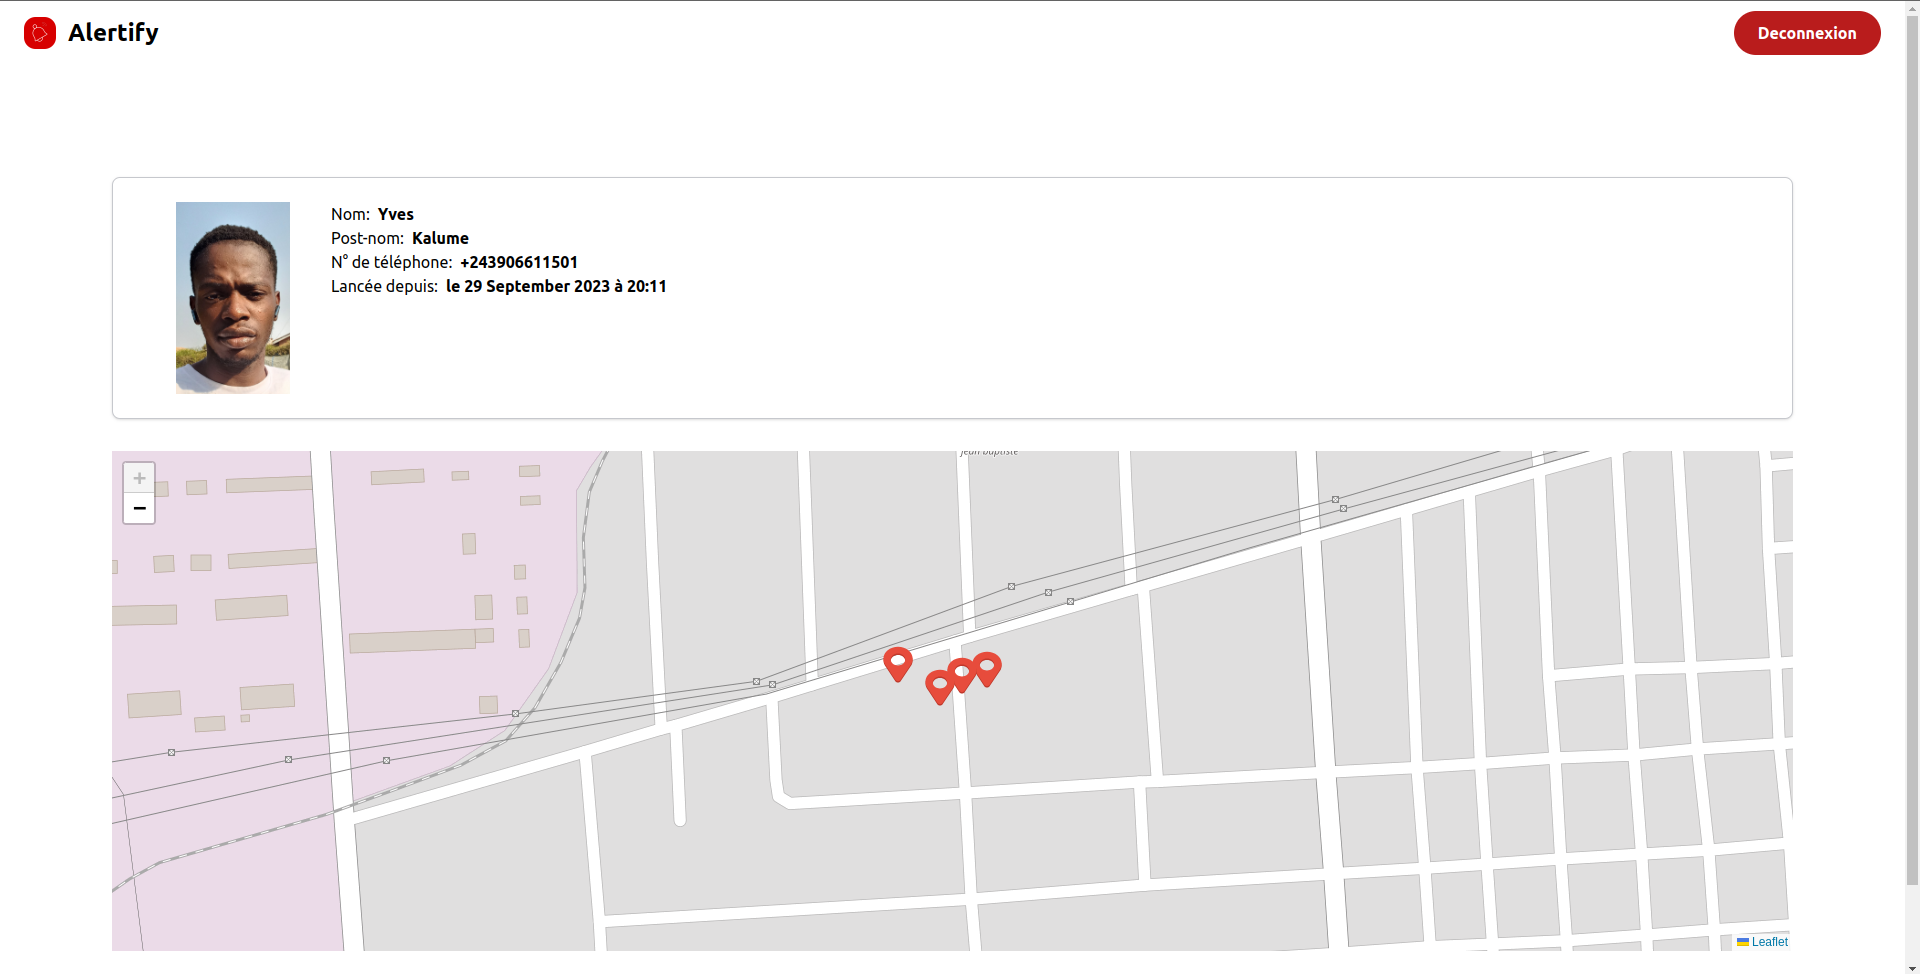
\includegraphics[width=\textwidth,frame]{admin_details}
	\caption{Détail d’une alerte}
\end{figure}

\section{Difficultés rencontrées}
Un travail scientifique vise toujours à résoudre un problème spécifique rencontré en apportant des solutions acceptables. C’est dans la recherche de cette solution que l’on oriente ses recherches dans un domaine bien déterminé et qu’on fixe les limites.

\begin{itemize}
	\item \textit{Manque d'informations des sources officielles }
\end{itemize}

Le manque d'informations fiables provenant de sources officielles a constitué un obstacle majeur. Les données sur les enlèvements, leur fréquence, leurs lieux et leurs circonstances étaient lacunaires et difficiles d'accès. Cela a compliqué notre travail d'analyse des tendances et d'adaptation de notre système aux besoins spécifiques de la ville de Lubumbashi. Nous avons dû recourir à des données disponibles, souvent limitées, et à des témoignages de la communauté locale pour informer notre approche.

\begin{itemize}
	\item \textit{Simulation de cas réels d’enlèvement}
\end{itemize}

Recréer fidèlement des cas réels d'enlèvement pour tester notre solution dans un contexte authentique s'est avéré une entreprise complexe, imprévisible et potentiellement dangereuse. La sécurité des participants est une priorité absolue, et la reproduction de situations de kidnapping authentiques implique des risques considérables. En conséquence, nous avons dû concevoir des méthodes alternatives de test qui garantissent la sécurité des participants tout en fournissant des résultats valables pour évaluer l'efficacité de notre système.\\

Ces difficultés ont mis à l'épreuve notre capacité à concevoir et à mettre en œuvre une solution efficace, tout en soulignant l'importance cruciale de l'adaptabilité et de la flexibilité pour répondre aux défis réels du terrain.

\section{ Conclusion partielle}
Ce chapitre a mis en lumière la mise en œuvre technique de notre système d'appel au secours dédié à la prévention des enlèvements dans la ville de Lubumbashi. Nous avons plongé dans les détails des algorithmes essentiels, des outils et des technologies utilisés. Au-delà des aspects techniques, nous avons également accordé une attention particulière à l'expérience utilisateur qui est un élément central pour garantir que notre solution est accessible, conviviale et efficace, enfin, nous avons parlé des défis que nous avons rencontrés et les solutions que nous avons apportées.
